
\documentclass[10pt]{article}
\usepackage[T1]{fontenc}
\usepackage[utf8]{inputenc}
\usepackage{helvet}
\renewcommand{\familydefault}{\sfdefault}
\usepackage[margin=0.78in,top=0.72in,bottom=0.72in]{geometry}
\usepackage{graphicx}
\usepackage{booktabs}
\usepackage{tabularx}
\usepackage{array}
\usepackage[table]{xcolor}
\usepackage{caption}
\usepackage{float}
\usepackage{fancyhdr}
\usepackage{hyperref}
\usepackage{microtype}
\usepackage{amsmath}
\definecolor{HeadingBlue}{HTML}{2E74B5}
\definecolor{DarkBlue}{HTML}{1F4D78}
\definecolor{Ink}{HTML}{17242A}
\definecolor{Muted}{HTML}{667280}
\definecolor{TableFill}{HTML}{E8EEF5}
\definecolor{CalloutFill}{HTML}{F4F6F9}
\definecolor{CautionFill}{HTML}{FFF7E6}
\definecolor{BorderColor}{HTML}{B8C2CC}
\hypersetup{colorlinks=true,linkcolor=DarkBlue,urlcolor=DarkBlue}
\captionsetup{font=small,labelfont=bf}
\setlength{\parindent}{0pt}
\setlength{\parskip}{0.45em}
\setlength{\arrayrulewidth}{0.35pt}
\renewcommand{\arraystretch}{1.18}
\pagestyle{fancy}
\fancyhf{}
\rhead{\footnotesize\textcolor{Muted}{DAMH ERT20 inversion report}}
\rfoot{\footnotesize\textcolor{Muted}{Page \thepage}}
\renewcommand{\headrulewidth}{0pt}
\renewcommand{\footrulewidth}{0pt}
\makeatletter
\renewcommand{\section}{\@startsection{section}{1}{0pt}{1.2em}{0.6em}{\large\bfseries\color{HeadingBlue}}}
\renewcommand{\subsection}{\@startsection{subsection}{2}{0pt}{0.9em}{0.4em}{\normalsize\bfseries\color{HeadingBlue}}}
\makeatother
\sloppy

\begin{document}

{\footnotesize\textcolor{Muted}{TECHNICAL REPORT}}\par
{\LARGE\bfseries DAMH ERT20 Fixed-Boundary Inversion}\par
{\normalsize\textcolor{Muted}{Compact technical record of time alignment, best fit, Archie calibration, and posterior diagnostics}}\par
\vspace{0.5em}

\begin{table}[H]
\centering
\small
\begin{tabularx}{\linewidth}{>{\raggedright\arraybackslash}p{0.29\linewidth} X}
\toprule
\rowcolor{TableFill}\textbf{Item} & \textbf{Value}\\
\midrule
Run & damh\_\allowbreak{}ert20\_\allowbreak{}t0\_\allowbreak{}fixed\_\allowbreak{}boundary\_\allowbreak{}deep\_\allowbreak{}su\_\allowbreak{}until\_\allowbreak{}20260614\_\allowbreak{}0800\_\allowbreak{}v1 \\
Config & ogs\_\allowbreak{}mh\_\allowbreak{}ert\_\allowbreak{}20point\_\allowbreak{}730d\_\allowbreak{}allparams\_\allowbreak{}per\_\allowbreak{}support\_\allowbreak{}archie\_\allowbreak{}recentered\_\allowbreak{}10h\_\allowbreak{}prior.json \\
Generated & 2026-06-14 18:07 local time from current run artifacts \\
Data used & ERT log10 resistivity only; 20 supports x 33 timestamps; no NMR, RH/suction, pressure, or deformation streams assimilated \\
Time window & 2019-12-23T02:00:00 to 2021-09-13T02:00:00 \\
\bottomrule
\end{tabularx}
\end{table}


\section*{Executive Summary}

\vspace{0.3em}
\noindent\fcolorbox{BorderColor}{CalloutFill}{%
\begin{minipage}{0.965\linewidth}
\small\textbf{Main record:} The inversion uses a fixed ERT-to-OGS time shift of 96.0817 d. This is a fixed alignment choice in the run, not a sampled posterior quantity. The open-niche boundary is also fixed: curve shift 0 d, suction scale 1, suction offset 0 MPa.
\end{minipage}}
\vspace{0.5em}


\begin{table}[H]
\centering
\small
\begin{tabularx}{\linewidth}{>{\raggedright\arraybackslash}p{0.29\linewidth} X}
\toprule
\rowcolor{TableFill}\textbf{Item} & \textbf{Value}\\
\midrule
Exact candidate sets & 1,840 \\
Combined training samples & 2,997 = 1,157 base + 1,840 exact DAMH \\
Observation vector & 660 values = 20 supports x 33 ERT timestamps \\
Feature count & 207 \\
Accepted posterior samples & 1753 accepted DAMH trace rows \\
Best data-fit candidate & solver01\_\allowbreak{}eval000014 \\
Posterior mode candidate & solver13\_\allowbreak{}eval000002 \\
Best-fit residual RMSE & 0.0343 \\
Best-fit standardized RMSE & 0.191 \\
\bottomrule
\end{tabularx}
\end{table}


\vspace{0.3em}
\noindent\fcolorbox{BorderColor}{CalloutFill}{%
\begin{minipage}{0.965\linewidth}
\small\textbf{Selection rule:} This compact report keeps figures that explain the inversion evidence: time alignment, fit quality, pointwise Archie behavior, parameter posterior-vs-prior checks, measurement posterior predictions, and one field-posterior summary. Production timing, rank housekeeping, full covariance matrices, and all per-point PDF dumps are intentionally left in the run directory.
\end{minipage}}
\vspace{0.5em}


\clearpage
\section*{Scope and Time Alignment}
We treat the ERT measurements as the only assimilated data stream. The observation operator compares support-averaged model response to log10 resistivity observations at 20 circular supports and 33 times. The shifted time axis is official ERT model day minus 96.0817 d, so the first ERT timestamp falls essentially at shifted OGS day 0. This convention is used consistently in the residual and posterior figures.


\begin{table}[H]
\centering
\small
\begin{tabularx}{\linewidth}{>{\raggedright\arraybackslash}p{0.29\linewidth} X}
\toprule
\rowcolor{TableFill}\textbf{Item} & \textbf{Value}\\
\midrule
Official ERT day 0 on shifted axis & -96.081672 d \\
Shifted OGS day 0 & 0 d \\
First shifted ERT day & 0.001661 d \\
Last shifted ERT day & 630.001661 d \\
Boundary pre-t0 construction & phase\_\allowbreak{}aligned\_\allowbreak{}scaled\_\allowbreak{}copy \\
Boundary at official ERT t0 & 8.193 MPa suction \\
Active boundary at shifted day 0 & 12.217 MPa suction \\
\bottomrule
\end{tabularx}
\end{table}


\begin{figure}[H]
\centering
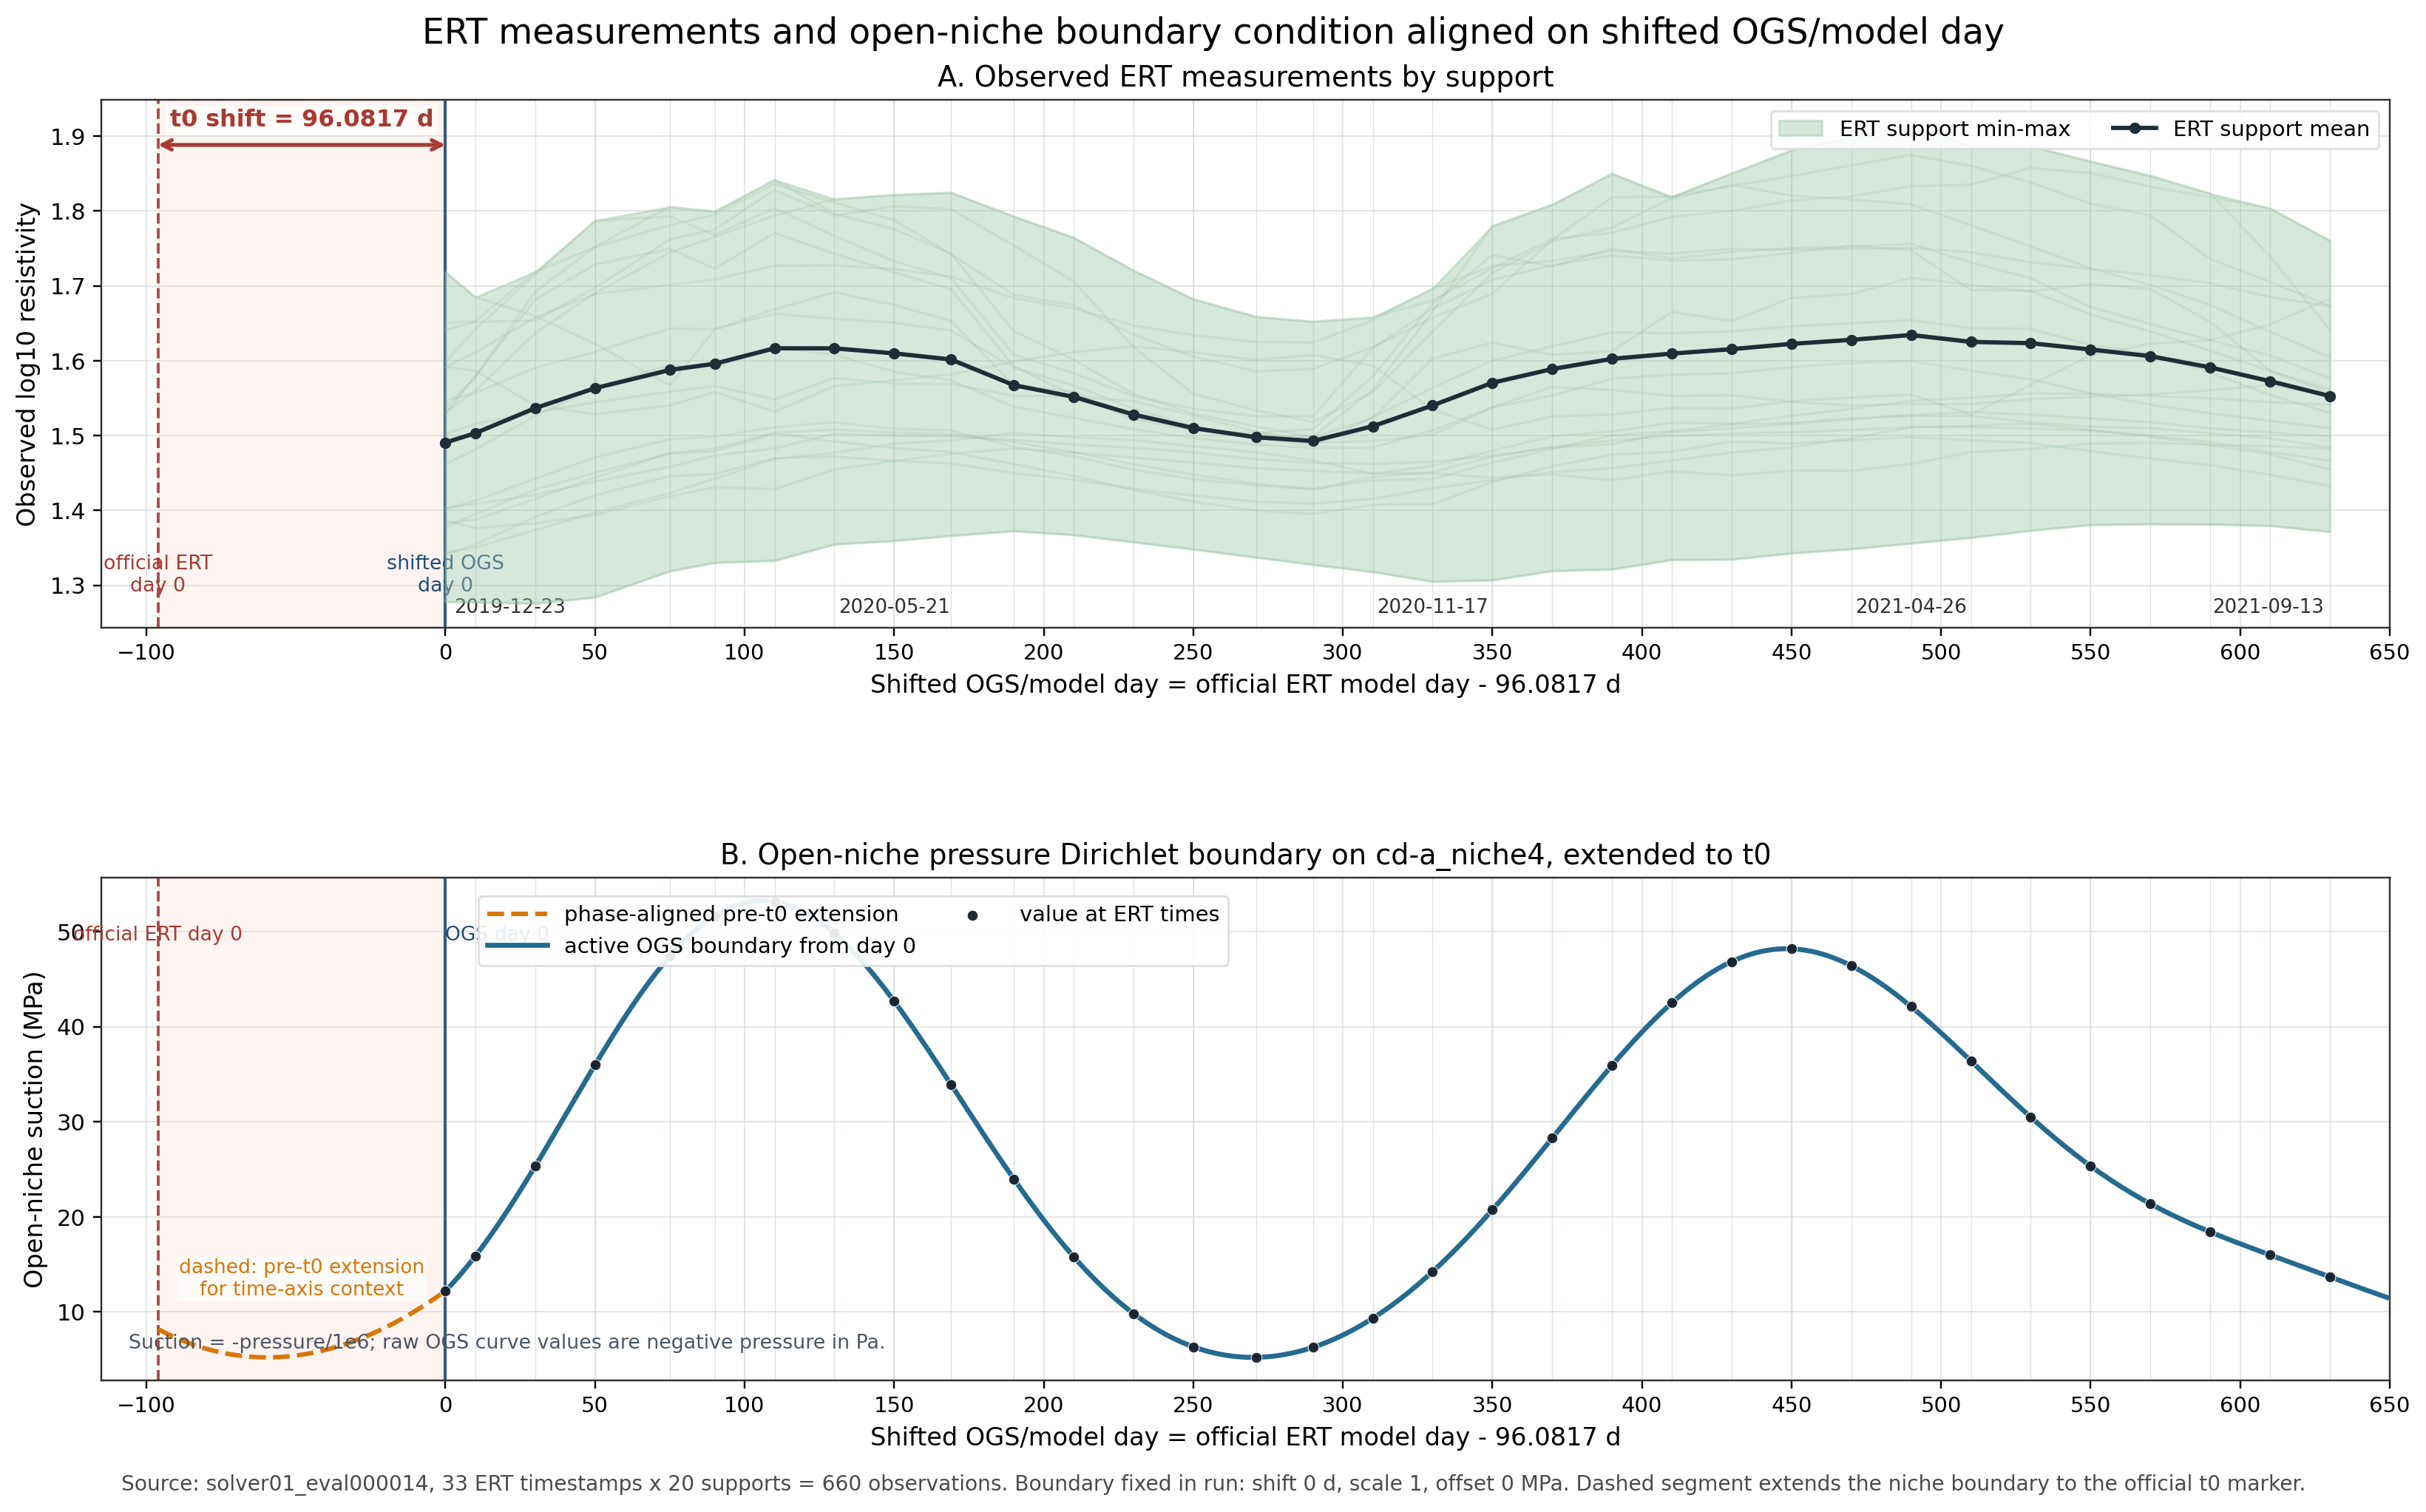
\includegraphics[width=\linewidth,height=0.72\textheight,keepaspectratio]{figures/timing/ert_measurements_open_niche_boundary_aligned_shifted_time_with_t0_shift.png}
\caption{ERT support envelope and fixed open-niche boundary on the same shifted time axis. The dashed pre-t0 segment is visual context and extends the boundary curve to official ERT day 0.}
\end{figure}


\clearpage
\section*{Run Design and Posterior Definition}
The run is a DAMH exact-candidate campaign using a surrogate-assisted proposal workflow. We use exact OGS candidate evaluations as the authoritative likelihood evidence. The posterior sample used here is empirical: accepted DAMH trace rows mapped to exact candidates, with rejected proposals and initial rank states excluded. This definition is useful for compact diagnostics, but it should not be read as an independent convergence proof.


\begin{table}[H]
\centering
\small
\begin{tabularx}{\linewidth}{>{\raggedright\arraybackslash}p{0.29\linewidth} X}
\toprule
\rowcolor{TableFill}\textbf{Item} & \textbf{Value}\\
\midrule
Manifest creation & 2026-06-13T22:07:21+02:00 \\
MPI size & 16 \\
DAMH trace rows & 1,825 \\
Accepted / rejected / prerejected & 1753 / 72 / 0 \\
Acceptance ratio & 0.9605 \\
Exact LL range & 60.53 to 62.21 \\
Timing audit & passed \\
\bottomrule
\end{tabularx}
\end{table}

\subsection*{Top Data-Fit Candidates}

\begin{table}[H]
\centering
\scriptsize
\resizebox{\linewidth}{!}{%
\begin{tabular}{l l l l l l l l}
\toprule
\rowcolor{TableFill}\textbf{Rank} & \textbf{Candidate} & \textbf{LL} & \textbf{MAE} & \textbf{log10 k0} & \textbf{Bedding} & \textbf{q22/q11} & \textbf{Porosity}\\
\midrule
1 & solver01\_\allowbreak{}eval000014 & 62.21 & 0.0245 & -21.37 & 141.1 & 0.423 & 0.15\\
2 & solver01\_\allowbreak{}eval000015 & 62.21 & 0.0245 & -21.42 & 141.3 & 0.418 & 0.149\\
3 & solver04\_\allowbreak{}eval000031 & 62.20 & 0.0248 & -21.11 & 139.4 & 0.369 & 0.15\\
4 & solver04\_\allowbreak{}eval000029 & 62.20 & 0.0248 & -21.07 & 139.8 & 0.373 & 0.149\\
5 & solver01\_\allowbreak{}eval000011 & 62.20 & 0.0245 & -21.31 & 140.2 & 0.452 & 0.152\\
6 & solver01\_\allowbreak{}eval000010 & 62.20 & 0.0244 & -21.27 & 140.2 & 0.453 & 0.147\\
7 & solver04\_\allowbreak{}eval000017 & 62.20 & 0.0245 & -20.95 & 139.5 & 0.417 & 0.136\\
8 & solver04\_\allowbreak{}eval000026 & 62.19 & 0.0249 & -20.89 & 139.9 & 0.383 & 0.144\\
\bottomrule
\end{tabular}}
\end{table}


\clearpage
\section*{Best Fit and Residual Structure}
The best data-fit candidate is solver01\_\allowbreak{}eval000014. Its local Archie objective is 0.036416, with residual MAE 0.02449, RMSE 0.03435, and standardized RMSE 0.19083. The residual mean is close to zero, so the main diagnostic question is spatial and temporal structure rather than an obvious global bias.


\begin{table}[H]
\centering
\small
\begin{tabularx}{\linewidth}{>{\raggedright\arraybackslash}p{0.29\linewidth} X}
\toprule
\rowcolor{TableFill}\textbf{Item} & \textbf{Value}\\
\midrule
Residual rows & 660 \\
Residual mean / median & -0.0001603 / 0.0004446 \\
Residual abs max & 0.18 \\
Standardized abs max & 0.998 \\
Support RMSE median & 0.0305 \\
Support RMSE max & 0.0617 \\
\bottomrule
\end{tabularx}
\end{table}


\begin{figure}[H]
\centering
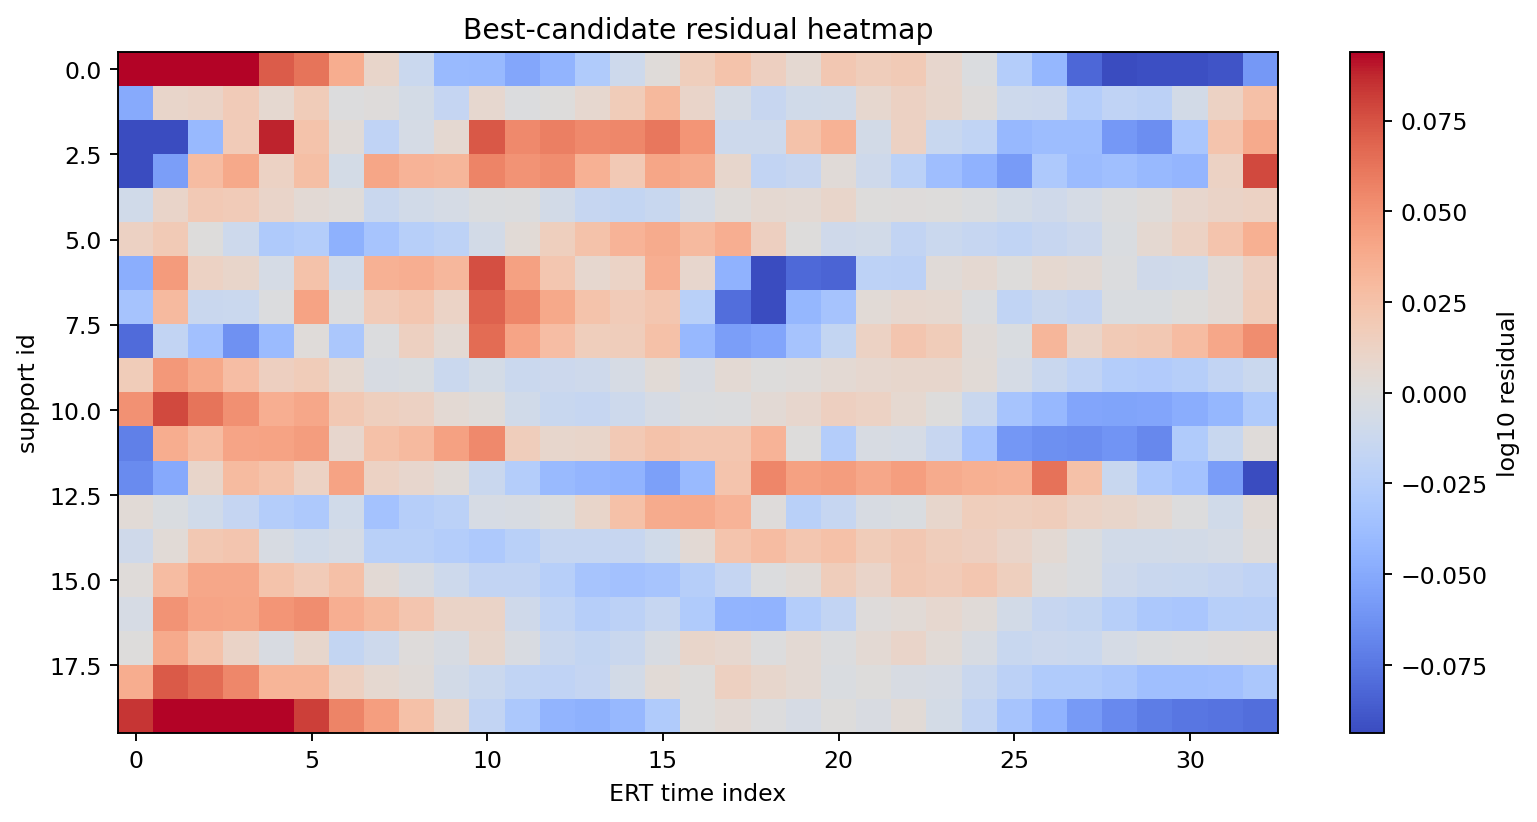
\includegraphics[width=\linewidth,height=0.50\textheight,keepaspectratio]{figures/07_best_candidate_residual_heatmap.png}
\caption{Best-candidate residuals by support and time after local Archie calibration.}
\end{figure}


\begin{figure}[H]
\centering
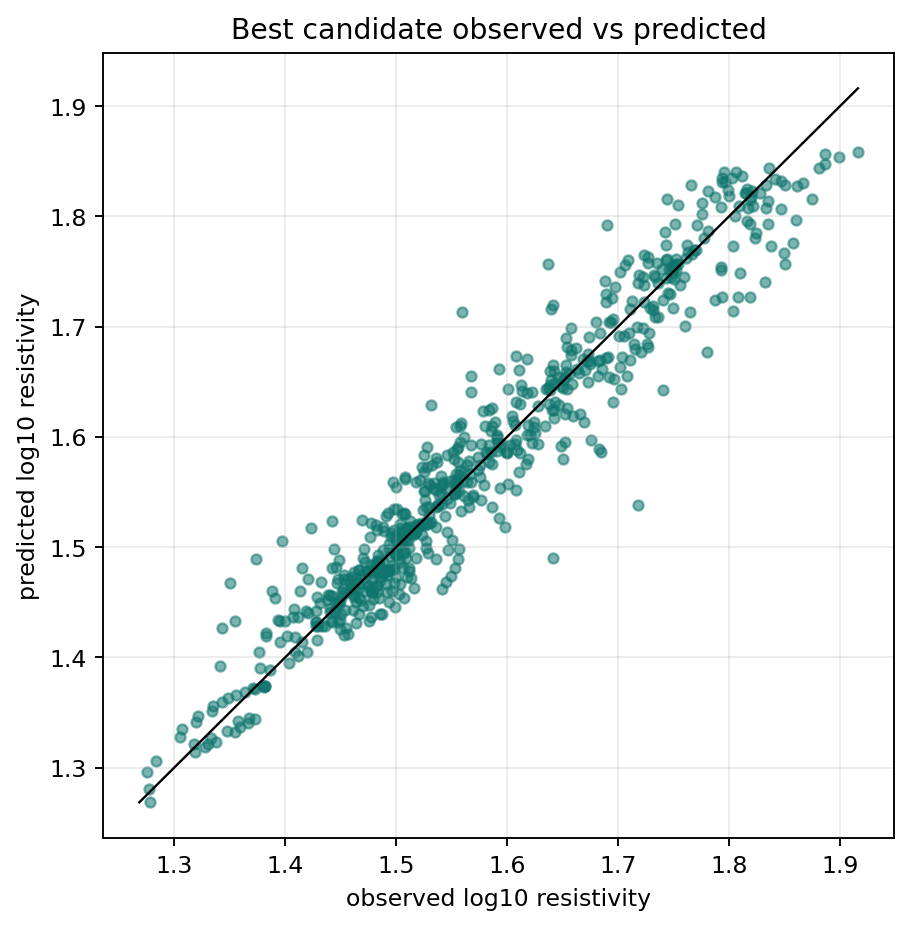
\includegraphics[width=\linewidth,height=0.62\textheight,keepaspectratio]{figures/08_best_candidate_observed_vs_predicted.png}
\caption{Observed versus predicted log10 resistivity for the best data-fit candidate.}
\end{figure}


\begin{figure}[H]
\centering
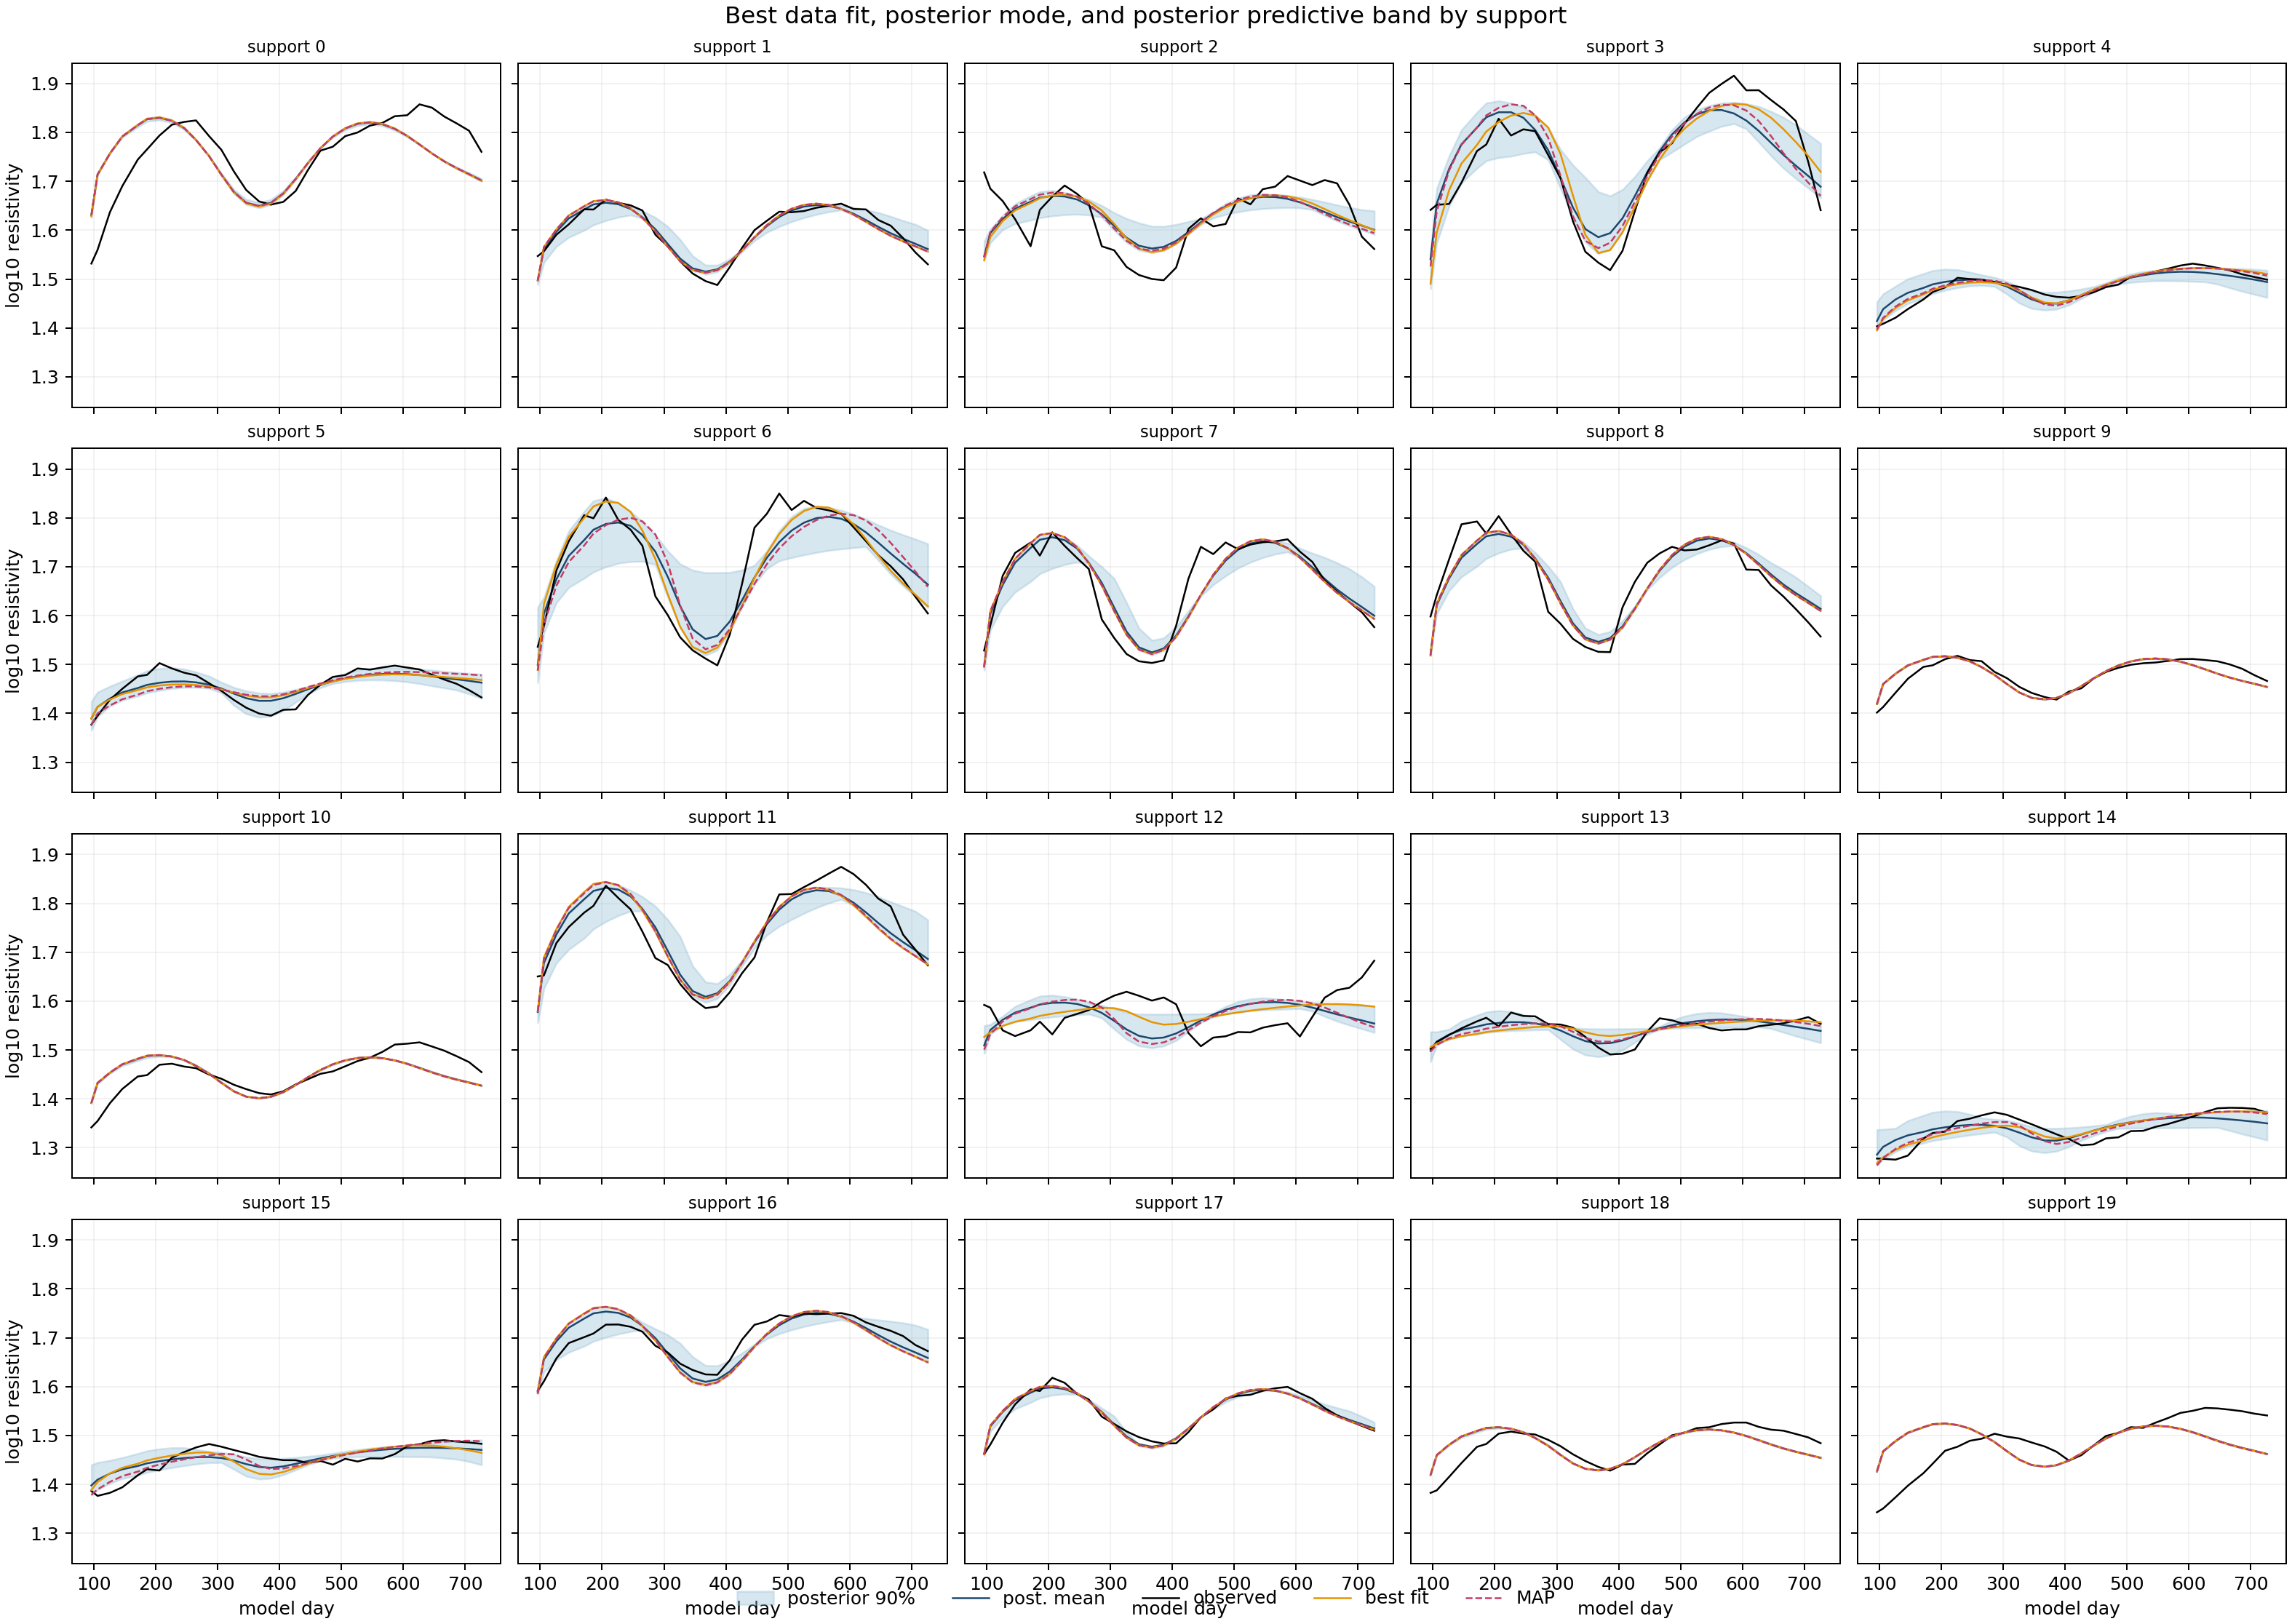
\includegraphics[width=\linewidth,height=0.68\textheight,keepaspectratio]{figures/posterior/posterior_best_fit_by_support_20plots.png}
\caption{Observed series, best fit, and posterior-mode comparison by ERT support.}
\end{figure}


\clearpage
\section*{Pointwise Archie Calibration}
The ERT comparison uses a local Archie-like transform per support. We therefore record support-level calibration rather than compressing it into a single global exponent. The fitted log10(a) and exponent b vary substantially around the niche, which is expected when a hydraulic state model is compared to electrical measurements through support-averaged transforms.


\begin{table}[H]
\centering
\small
\resizebox{\linewidth}{!}{%
\begin{tabular}{l l l l l l}
\toprule
\rowcolor{TableFill}\textbf{Archie quantity} & \textbf{Mean} & \textbf{Std} & \textbf{Min} & \textbf{Median} & \textbf{Max}\\
\midrule
log10(a) & 1.001 & 0.39 & -0.143 & 1.162 & 1.300\\
exponent b & -0.572 & 0.453 & -2.000 & -0.436 & -0.2\\
\bottomrule
\end{tabular}}
\end{table}


\begin{figure}[H]
\centering
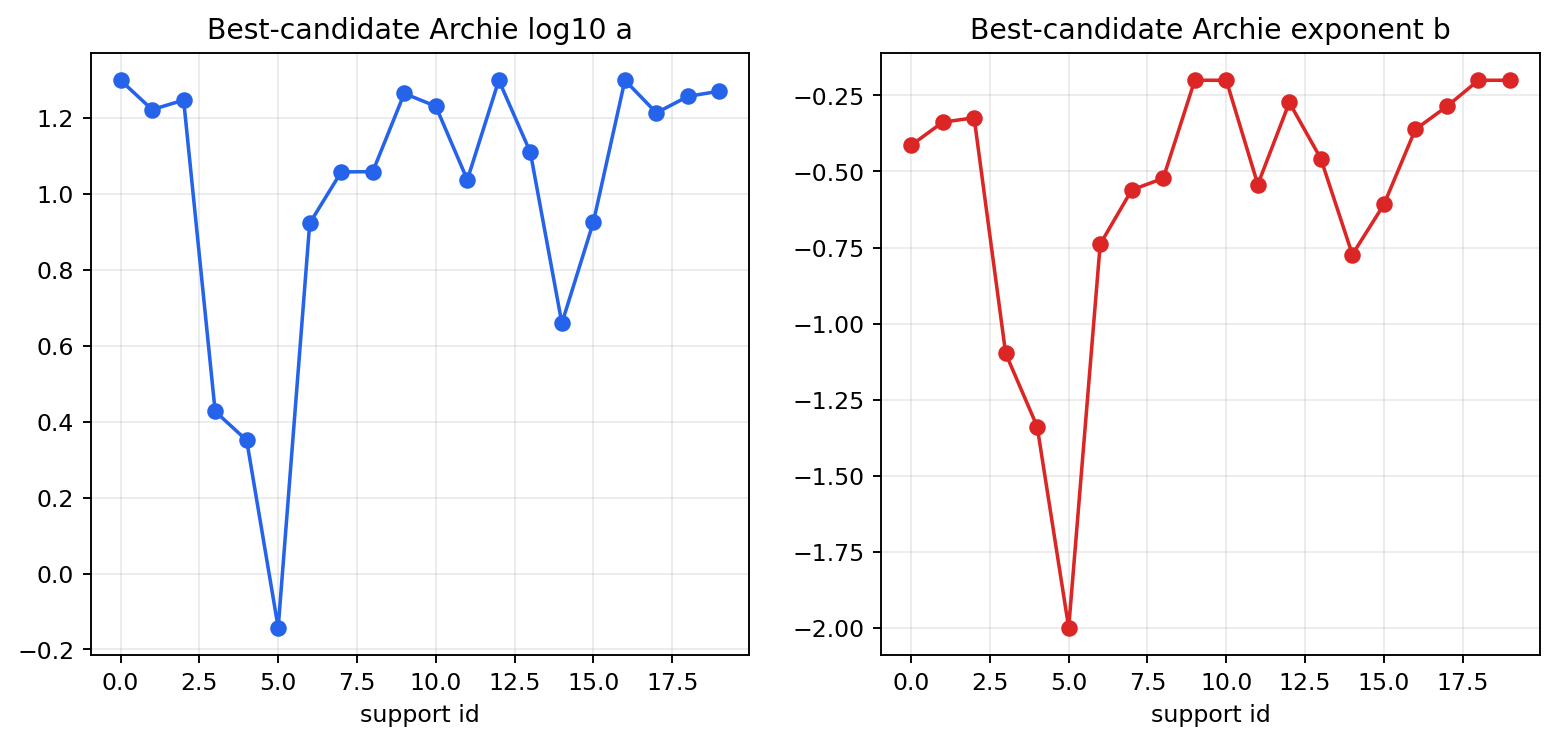
\includegraphics[width=\linewidth,height=0.50\textheight,keepaspectratio]{figures/09_best_candidate_archie_params.png}
\caption{Best-candidate fitted Archie parameters by support.}
\end{figure}


\begin{figure}[H]
\centering
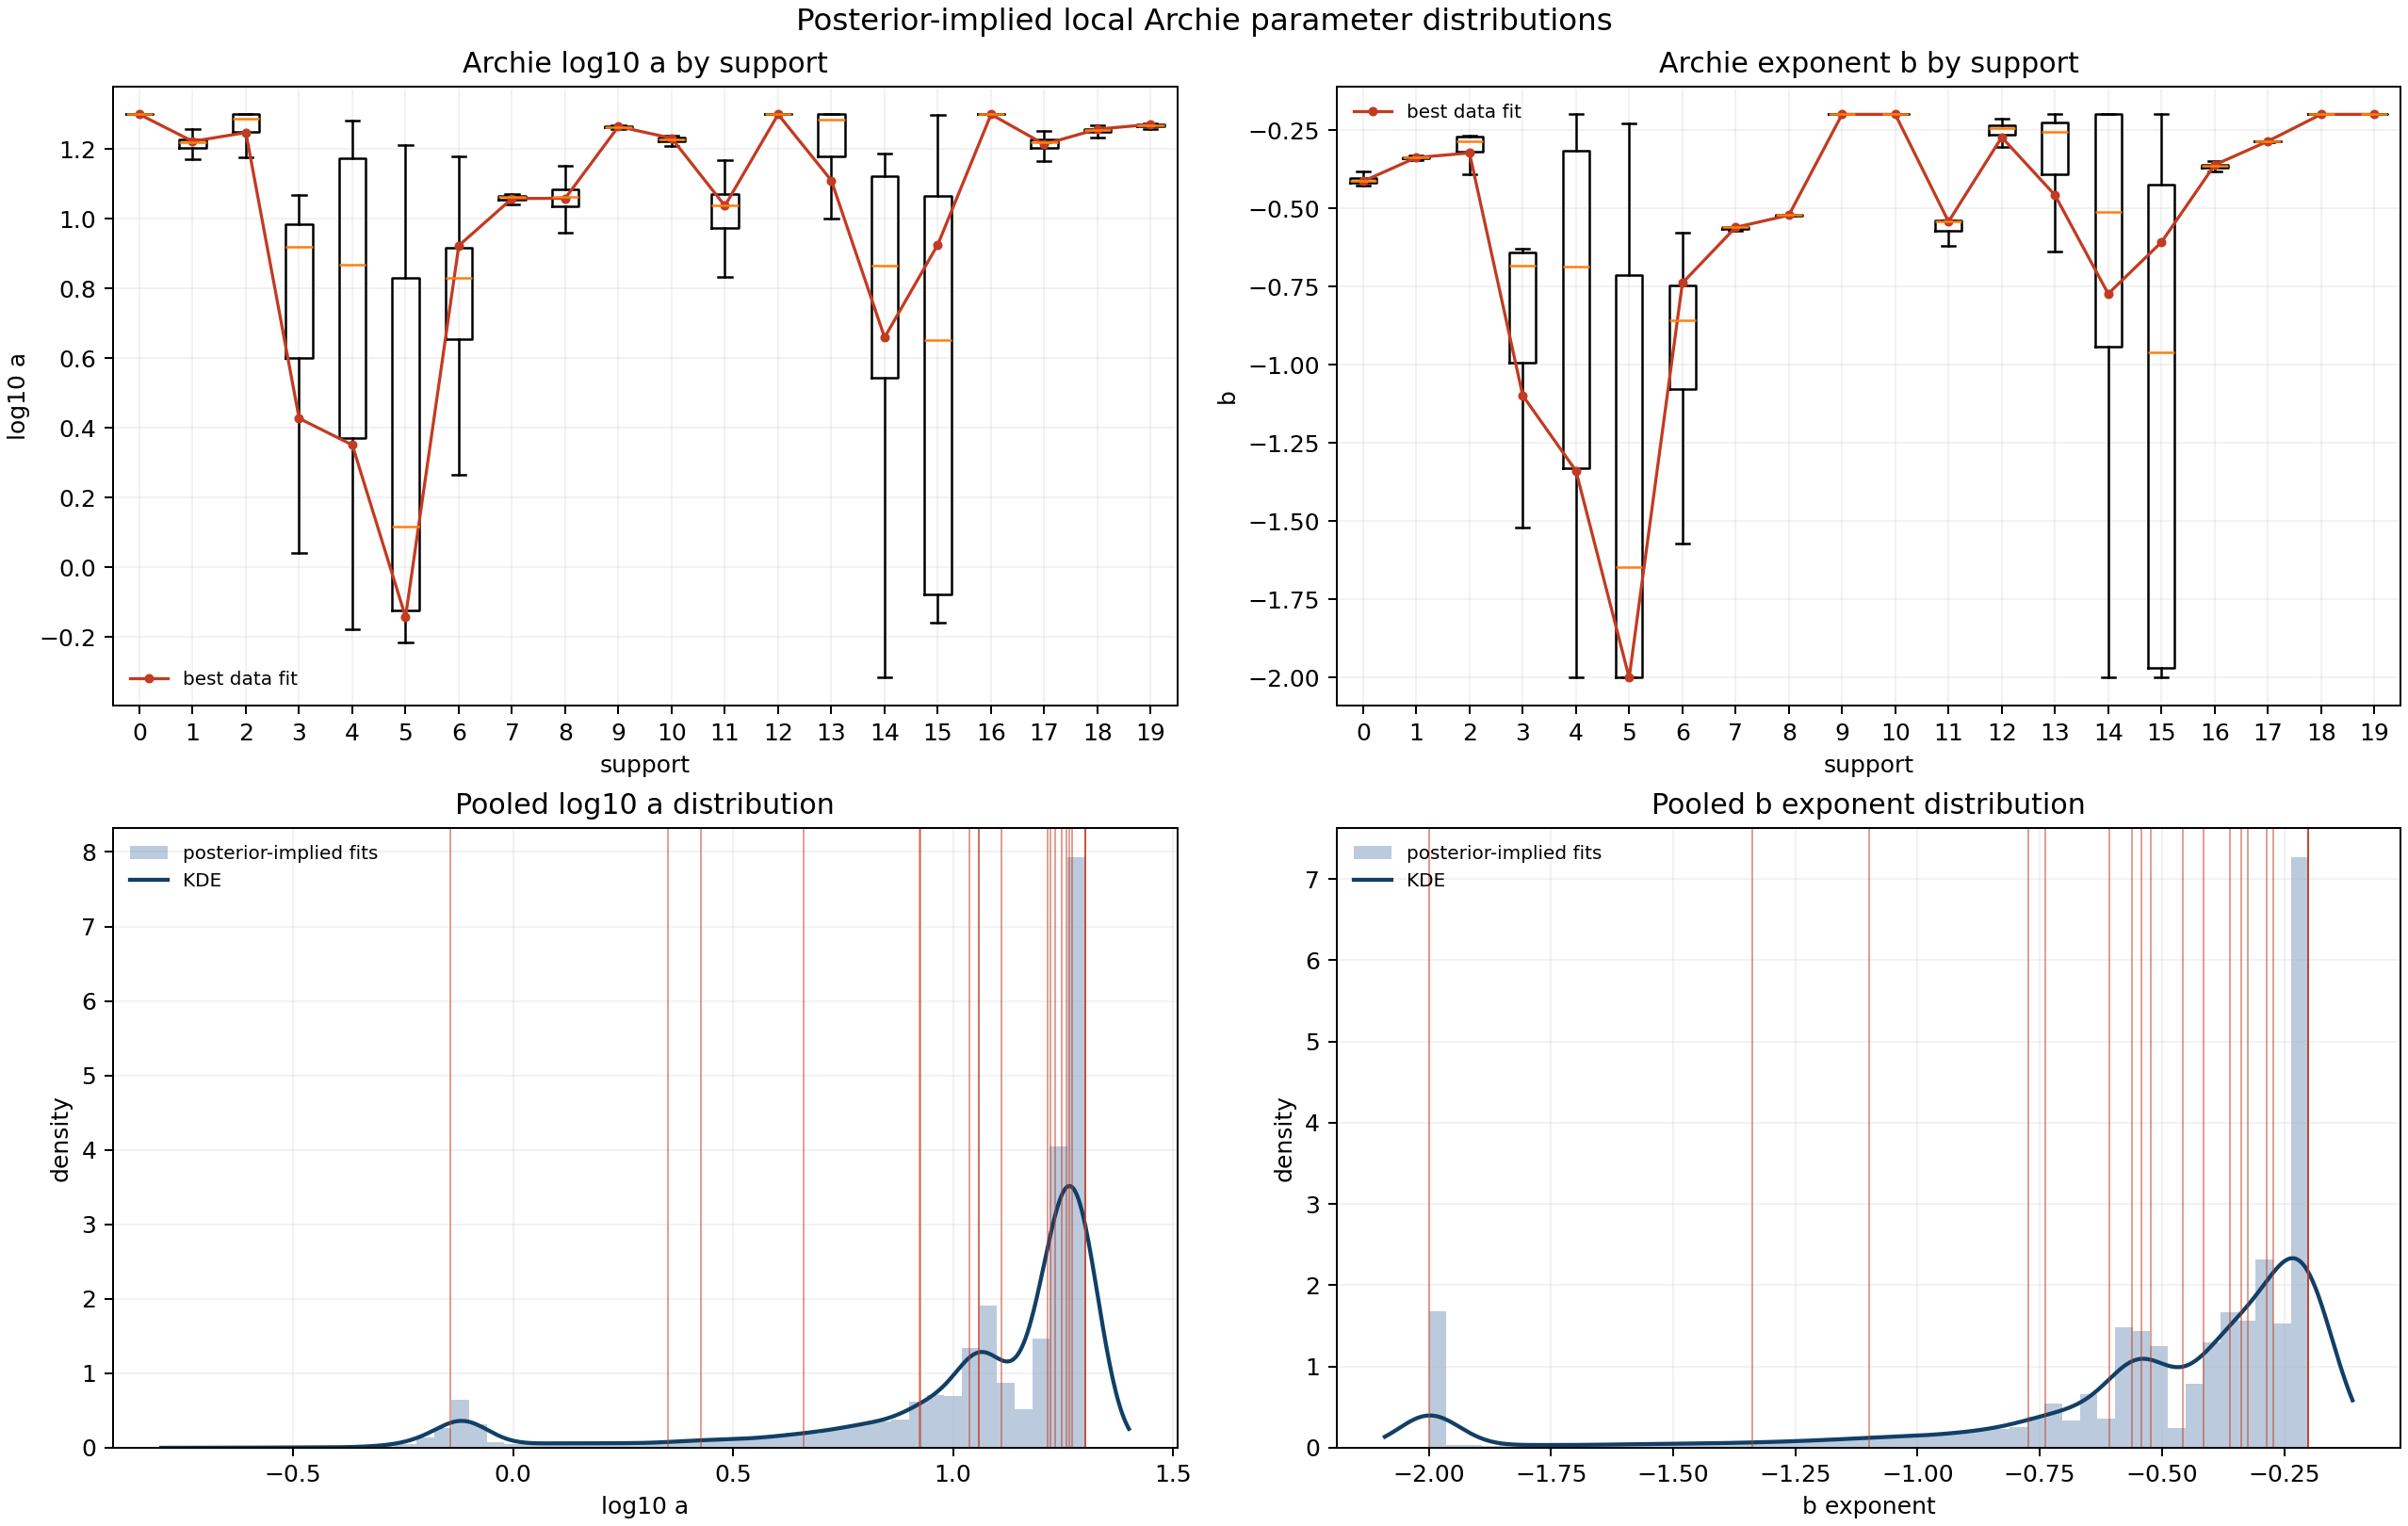
\includegraphics[width=\linewidth,height=0.63\textheight,keepaspectratio]{figures/posterior/posterior_archie_distributions.png}
\caption{Posterior distribution of local Archie coefficients across accepted DAMH trace samples.}
\end{figure}


\clearpage
\section*{Parameter Posteriors Against Priors}
The scalar posterior summaries separate material and observation-alignment decisions. The permeability scale, bedding angle, anisotropy ratio, and homogeneous porosity are sampled parameters. The open-niche boundary parameters are listed for traceability, but they are fixed in this run; their zero posterior variance is a policy choice, not information learned from ERT.


\begin{table}[H]
\centering
\tiny
\resizebox{\linewidth}{!}{%
\begin{tabular}{l l l l l l}
\toprule
\rowcolor{TableFill}\textbf{Parameter} & \textbf{Prior} & \textbf{Posterior summary} & \textbf{Best} & \textbf{Mode} & \textbf{Comment}\\
\midrule
Base log10 permeability & normal; mean -21.02, sd 5.100 & -20.94 +/- 1.300; 5-50-95\% -23.21, -20.84, -18.91 & -21.37 & -21.11 & \\
Bedding angle & normal; mean 139.9, sd 5.000 & 139.3 +/- 1.994; 5-50-95\% 135.9, 139.3, 142.8 & 141.1 & 139.8 & \\
Anisotropy q22/q11 & uniform 0.1..0.9 & 0.444 +/- 0.0636; 5-50-95\% 0.327, 0.45, 0.538 & 0.423 & 0.443 & \\
Homogeneous porosity & truncated\_\allowbreak{}normal; mean 0.15, sd 0.012 & 0.149 +/- 0.00857; 5-50-95\% 0.135, 0.149, 0.164 & 0.15 & 0.153 & \\
Niche shift & truncated\_\allowbreak{}normal; mean 92.09, sd 35.00, bounds 0..260.0 & 0 +/- 0; 5-50-95\% 0, 0, 0 & 0 & 0 & Fixed in this run; posterior is degenerate.\\
Niche suction scale & truncated\_\allowbreak{}normal; mean 1.230, sd 0.15, bounds 0.65..1.350 & 1.000 +/- 0; 5-50-95\% 1.000, 1.000, 1.000 & 1.000 & 1.000 & Fixed in this run; posterior is degenerate.\\
Niche suction offset & truncated\_\allowbreak{}normal; mean 0.243, sd 0.6, bounds -2.000..2.000 & 0 +/- 0; 5-50-95\% 0, 0, 0 & 0 & 0 & Fixed in this run; posterior is degenerate.\\
\bottomrule
\end{tabular}}
\end{table}


\begin{figure}[H]
\centering
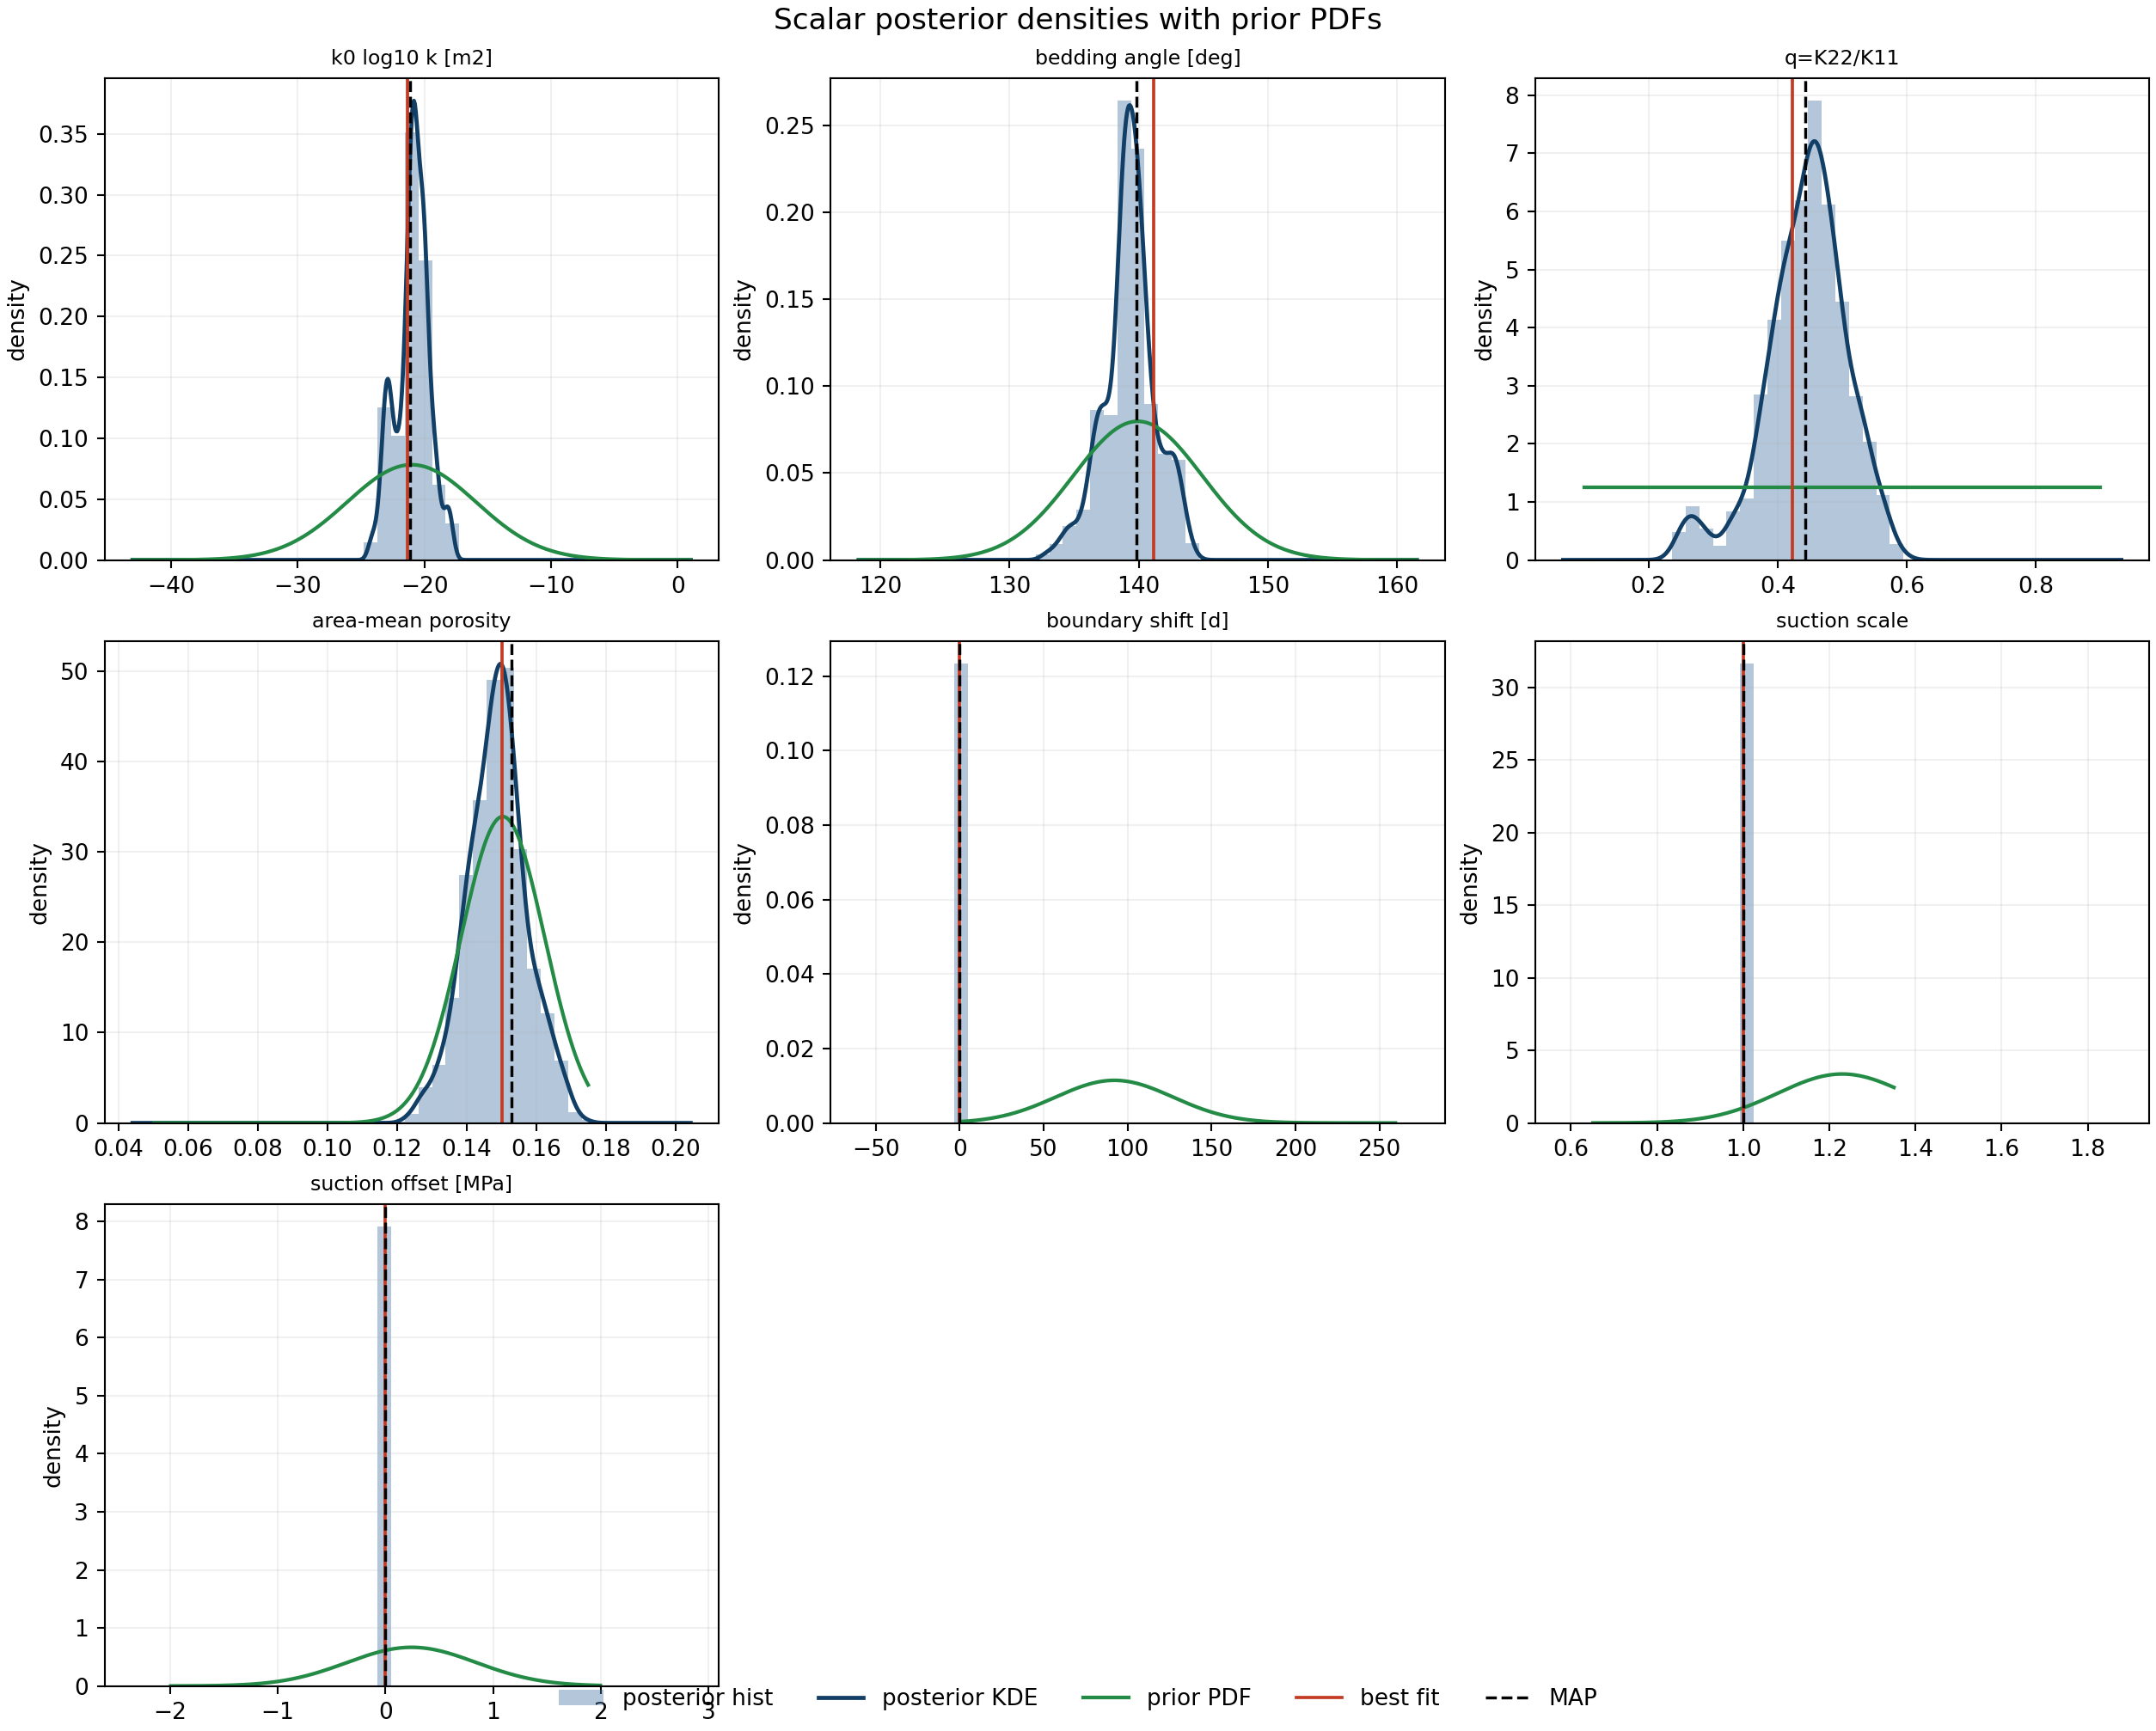
\includegraphics[width=\linewidth,height=0.71\textheight,keepaspectratio]{figures/posterior/posterior_scalar_prior_kde.png}
\caption{Posterior scalar parameter marginals against their priors.}
\end{figure}


\begin{figure}[H]
\centering
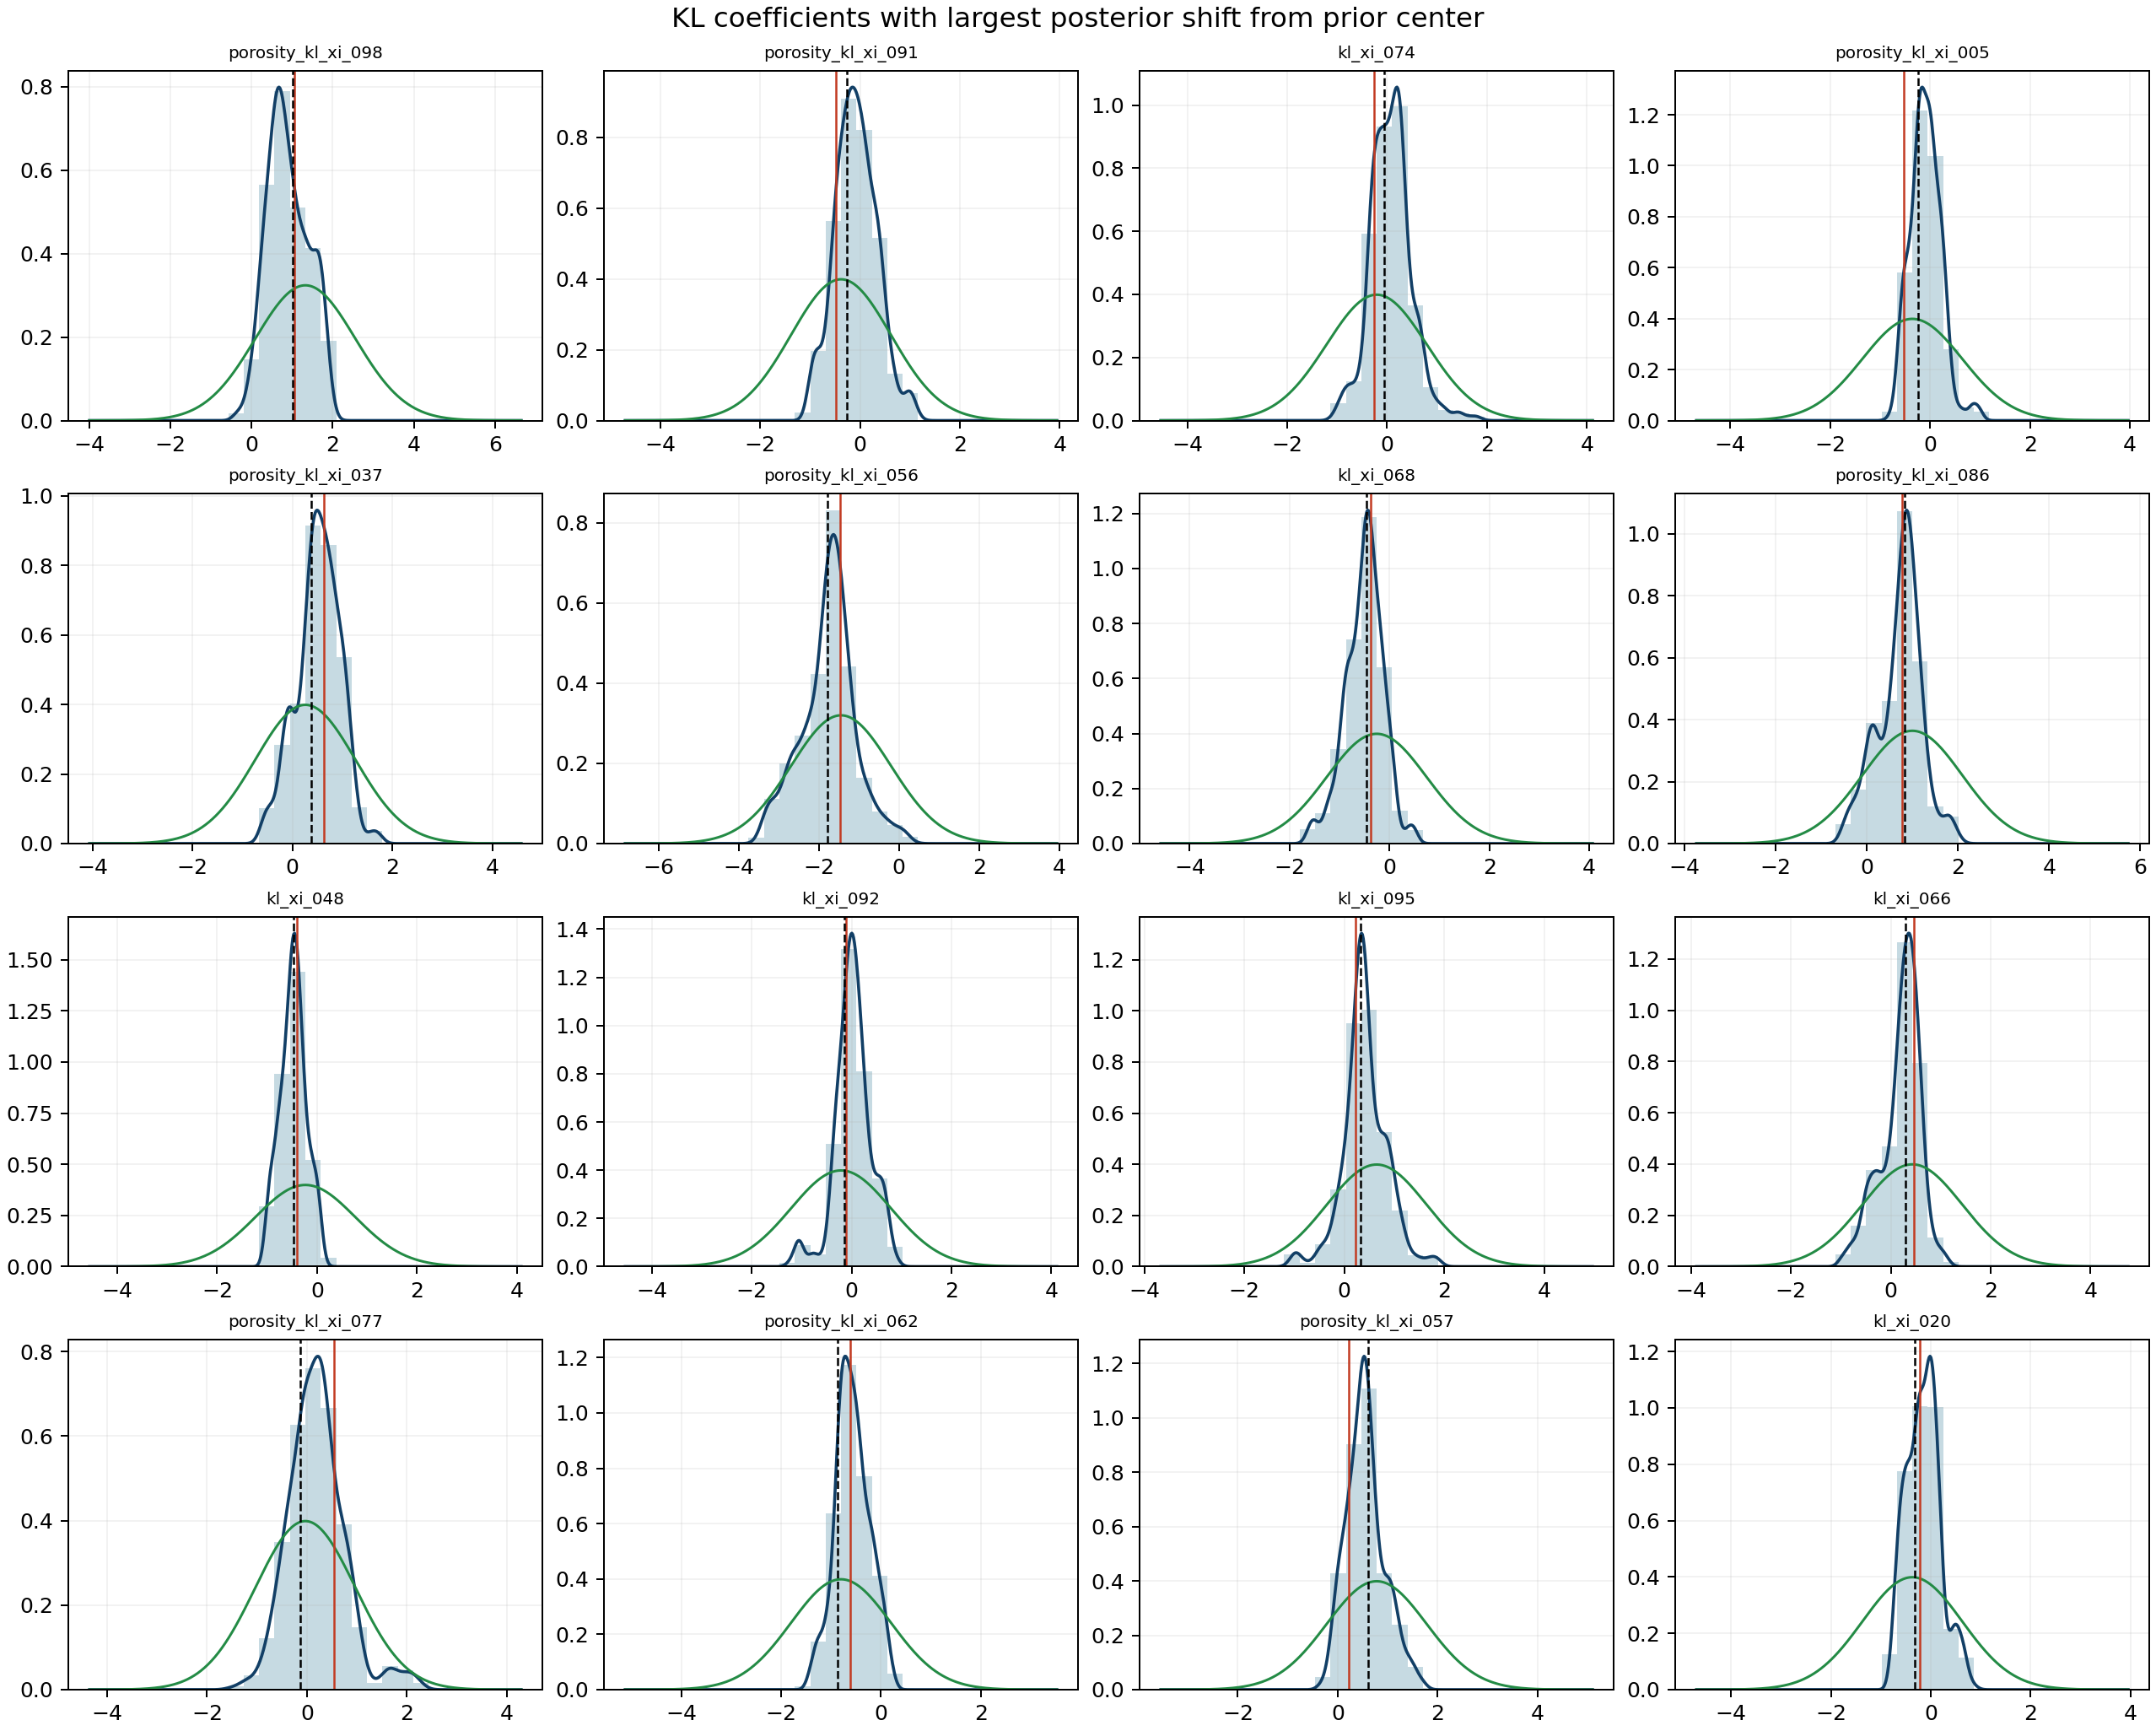
\includegraphics[width=\linewidth,height=0.71\textheight,keepaspectratio]{figures/posterior/posterior_top_kl_prior_kde.png}
\caption{Highest-information KL-style coefficients shown against their priors.}
\end{figure}


\clearpage
\section*{Posterior at Measurements}
Posterior predictive diagnostics are evaluated at the same 660 ERT support-time measurements used in the objective. We include density views rather than every per-point plot: this records whether the accepted candidate cloud covers the observations while keeping the report readable. Measurement-noise PDFs remain support-specific and are shown as a separate calibration reference.


\begin{figure}[H]
\centering
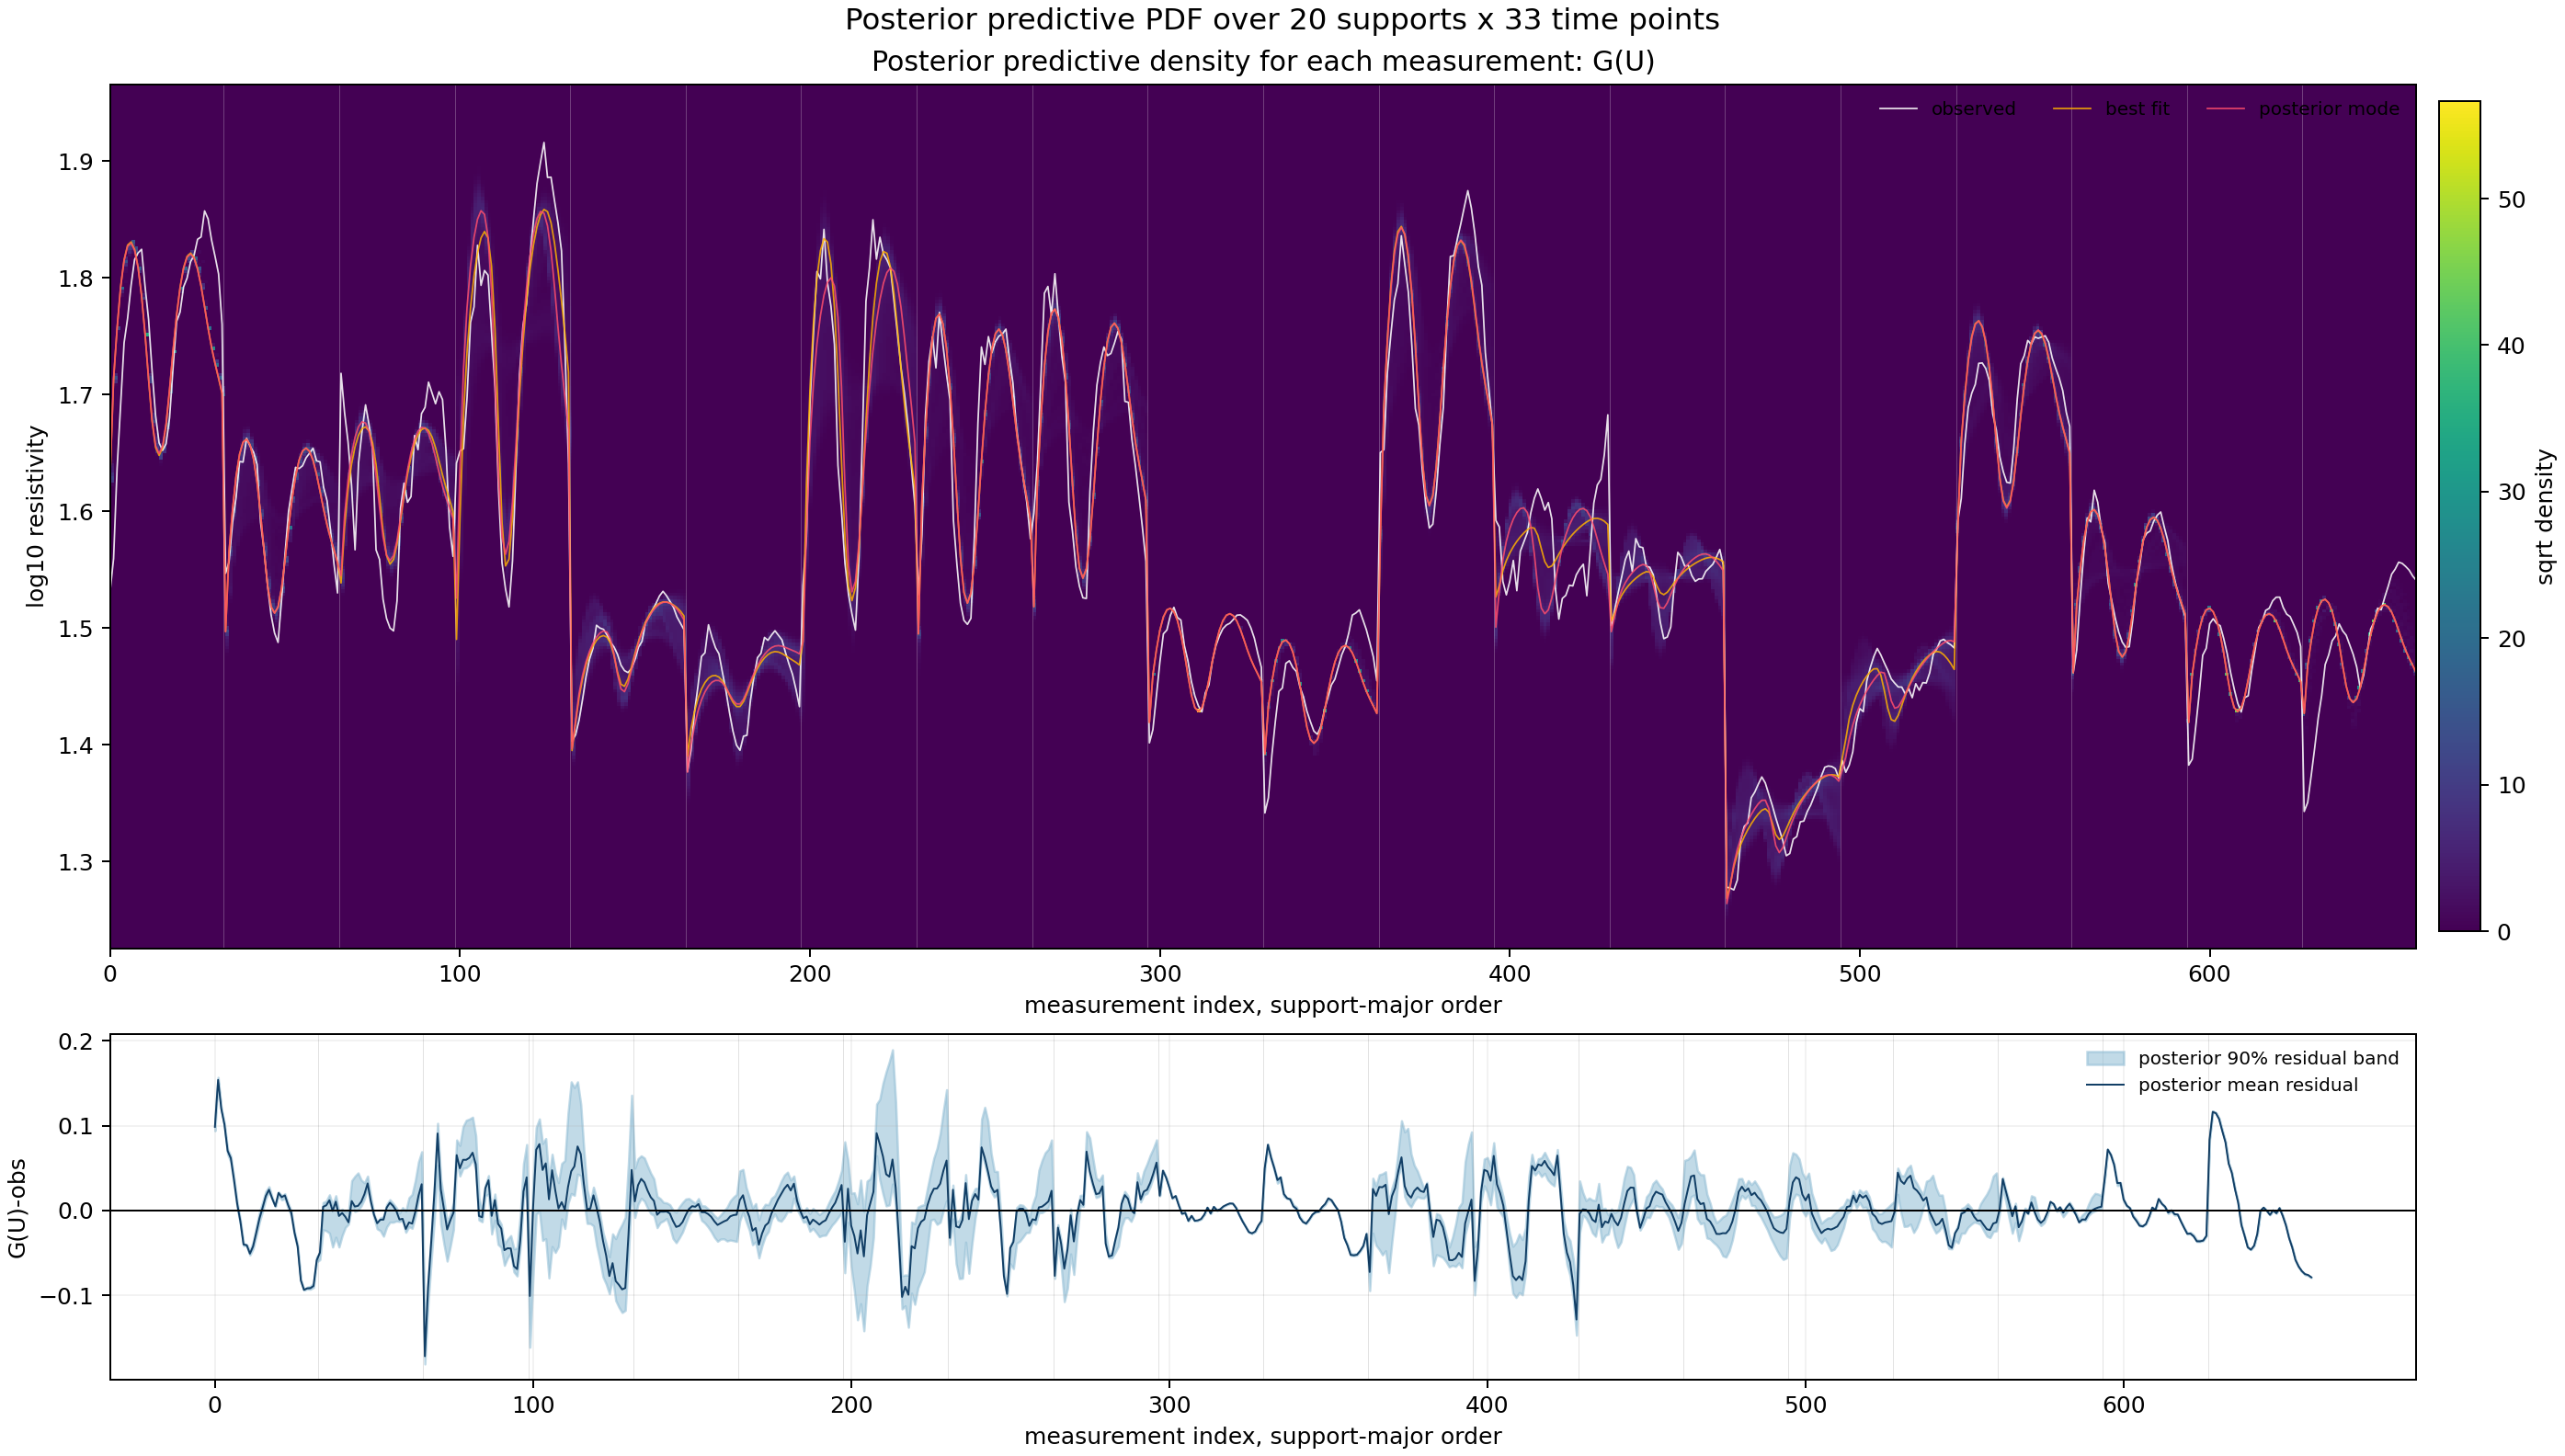
\includegraphics[width=\linewidth,height=0.58\textheight,keepaspectratio]{figures/posterior/posterior_predictive_density_by_measurement.png}
\caption{Posterior predictive density at measurement locations and times.}
\end{figure}


\begin{figure}[H]
\centering
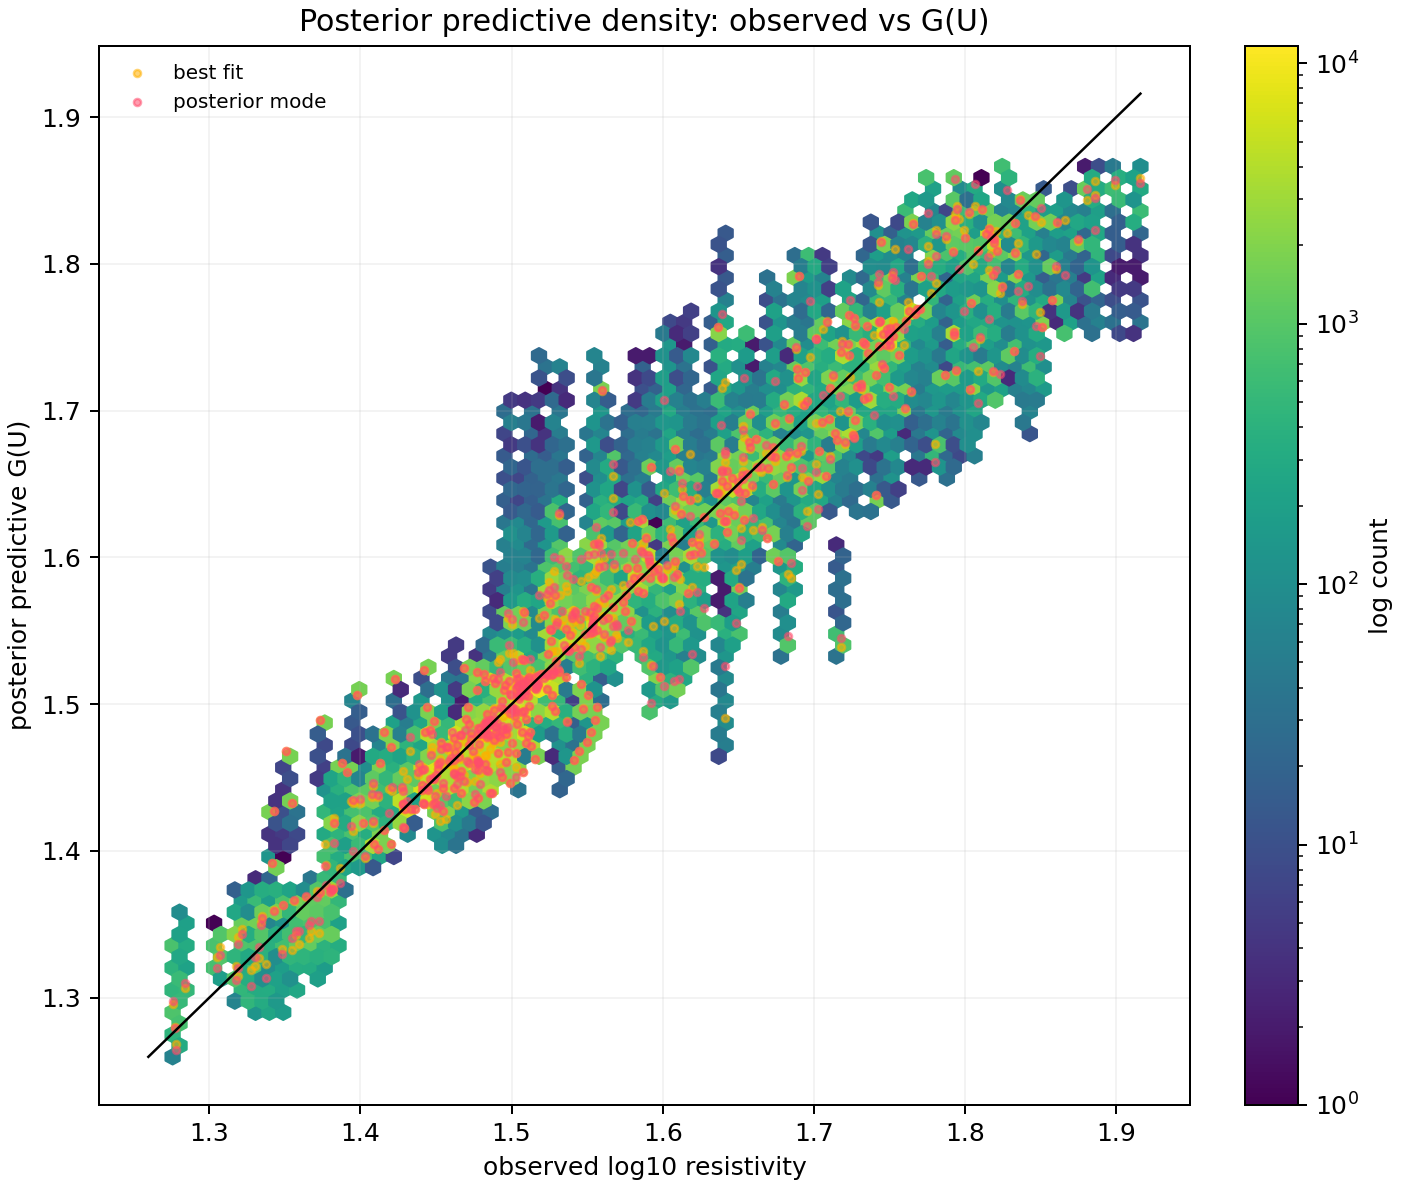
\includegraphics[width=\linewidth,height=0.65\textheight,keepaspectratio]{figures/posterior/posterior_predictive_observed_vs_gu_density.png}
\caption{Observed versus posterior predictive density in GU/log10-resistivity space.}
\end{figure}


\begin{figure}[H]
\centering
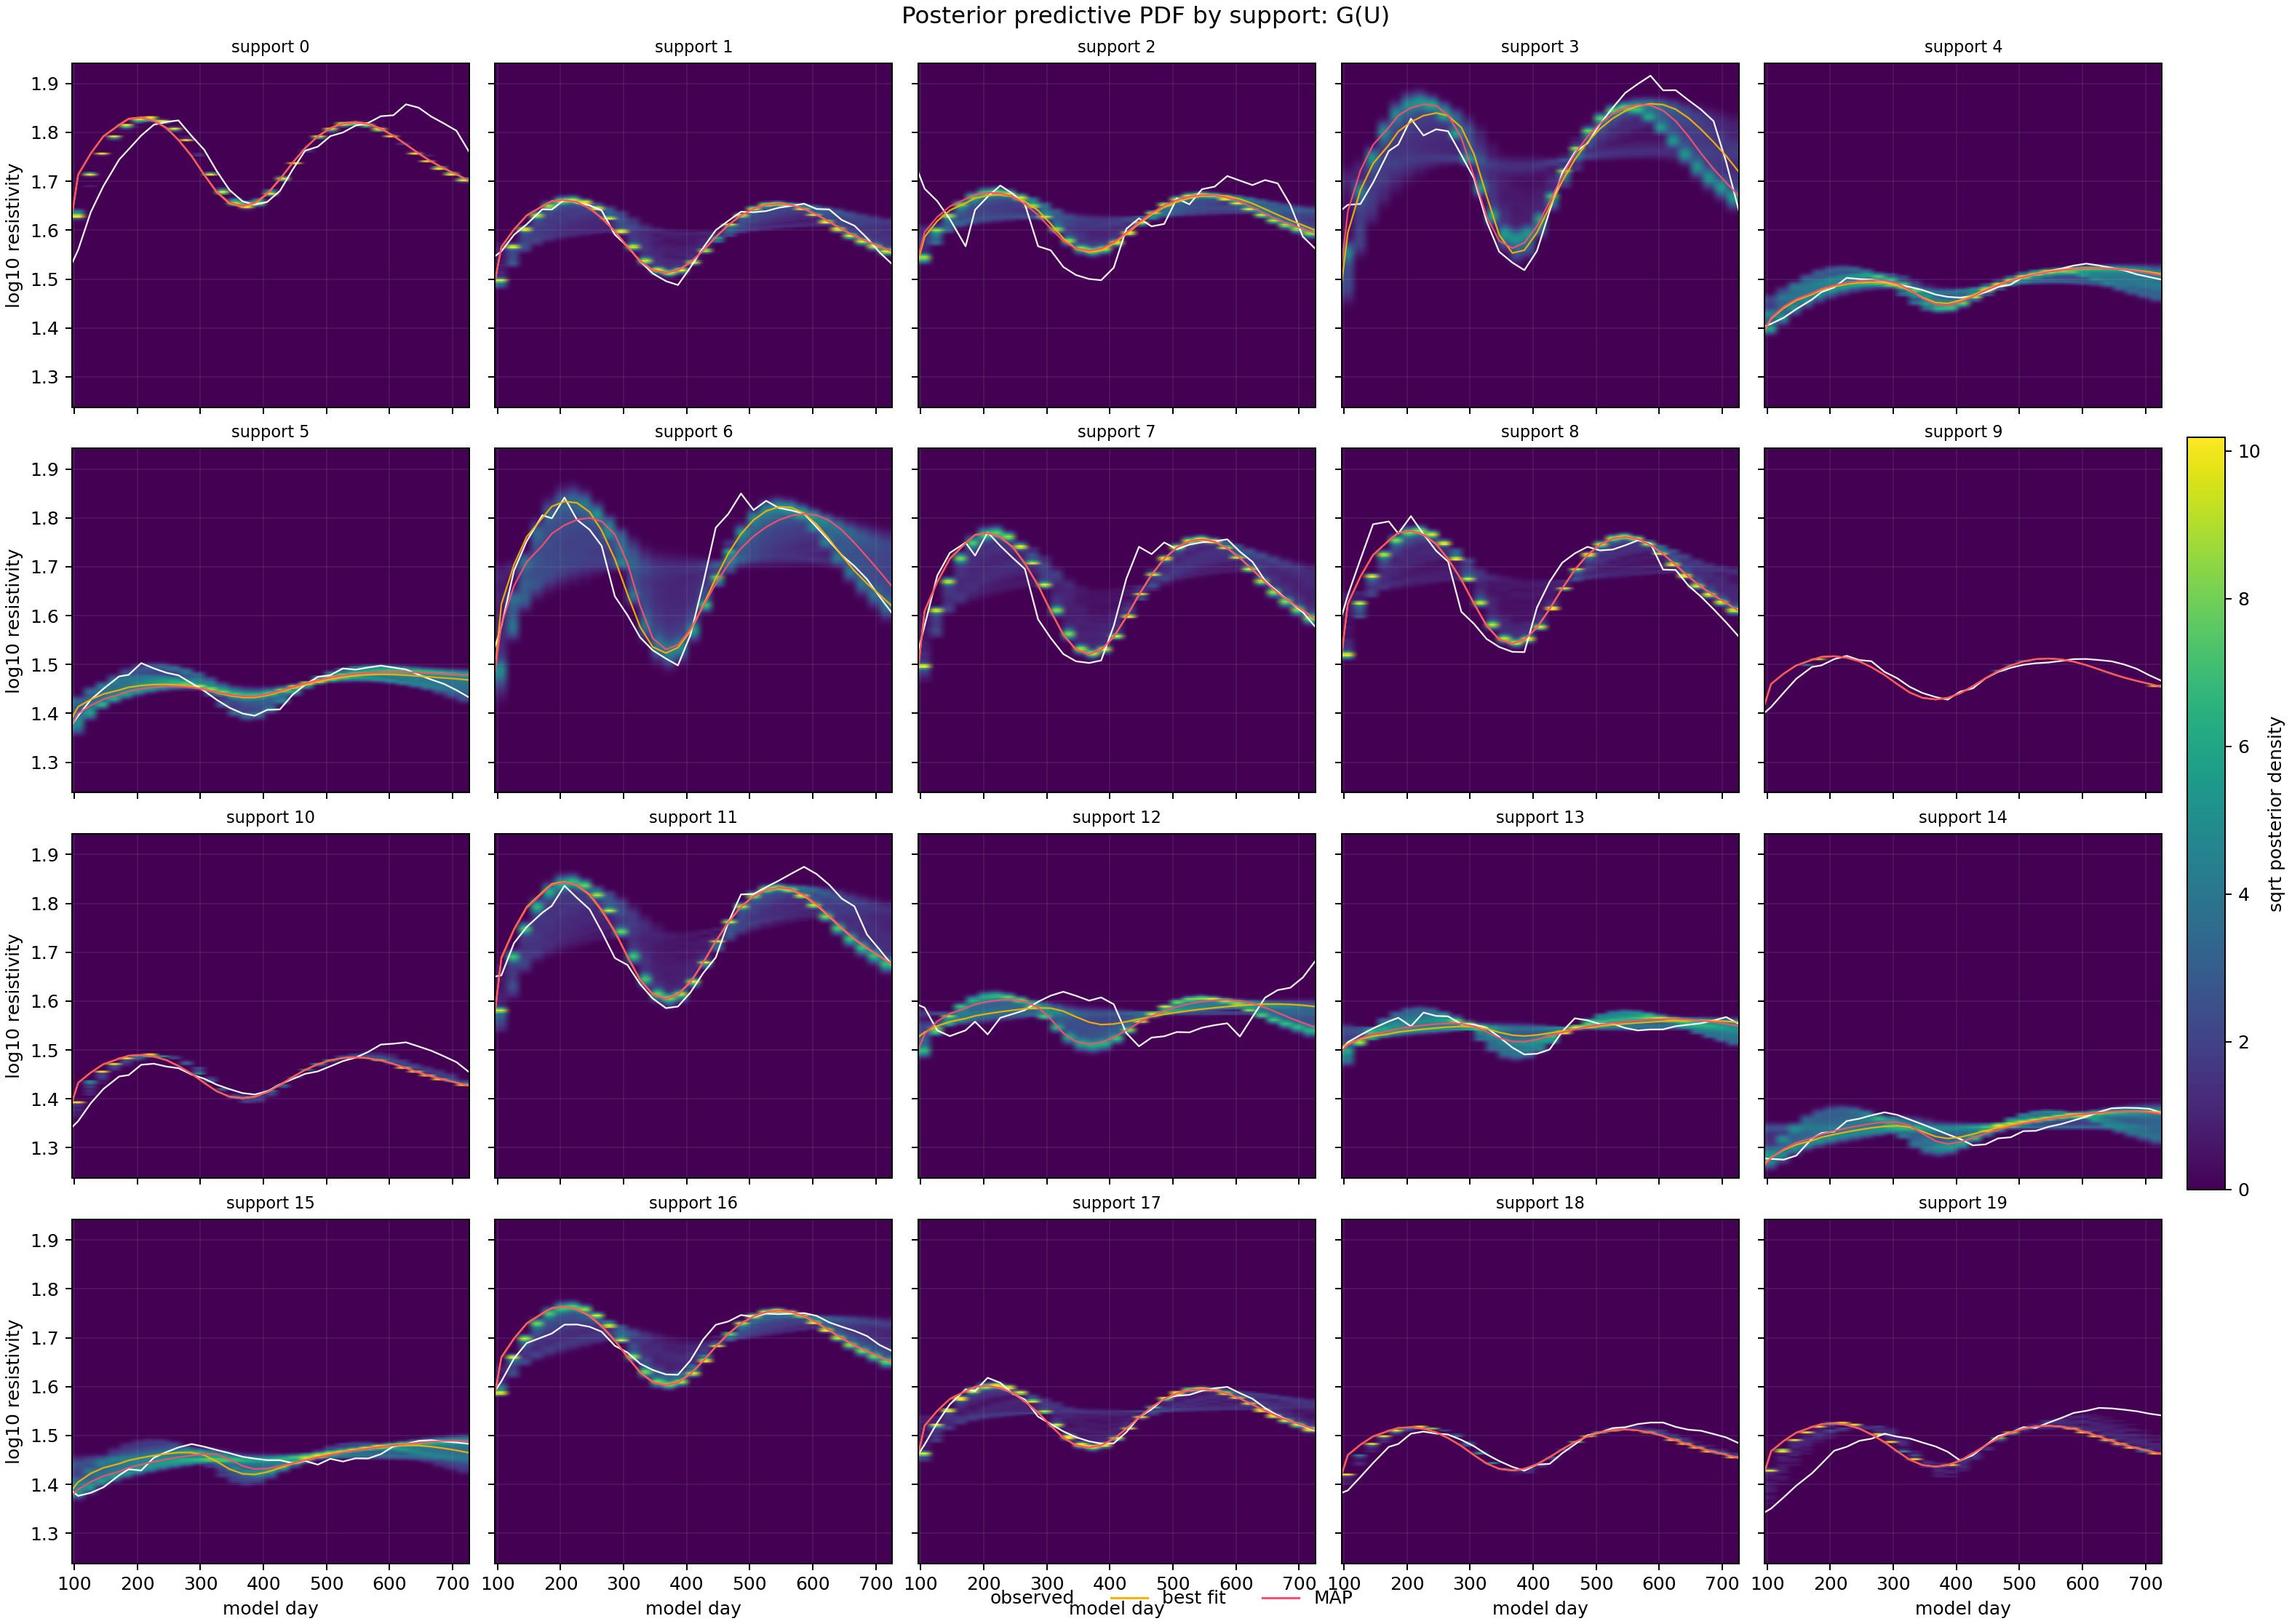
\includegraphics[width=\linewidth,height=0.70\textheight,keepaspectratio]{figures/posterior/posterior_predictive_pdf_by_support_20plots.png}
\caption{Posterior predictive PDFs by support, compact 20-panel view.}
\end{figure}


\begin{figure}[H]
\centering
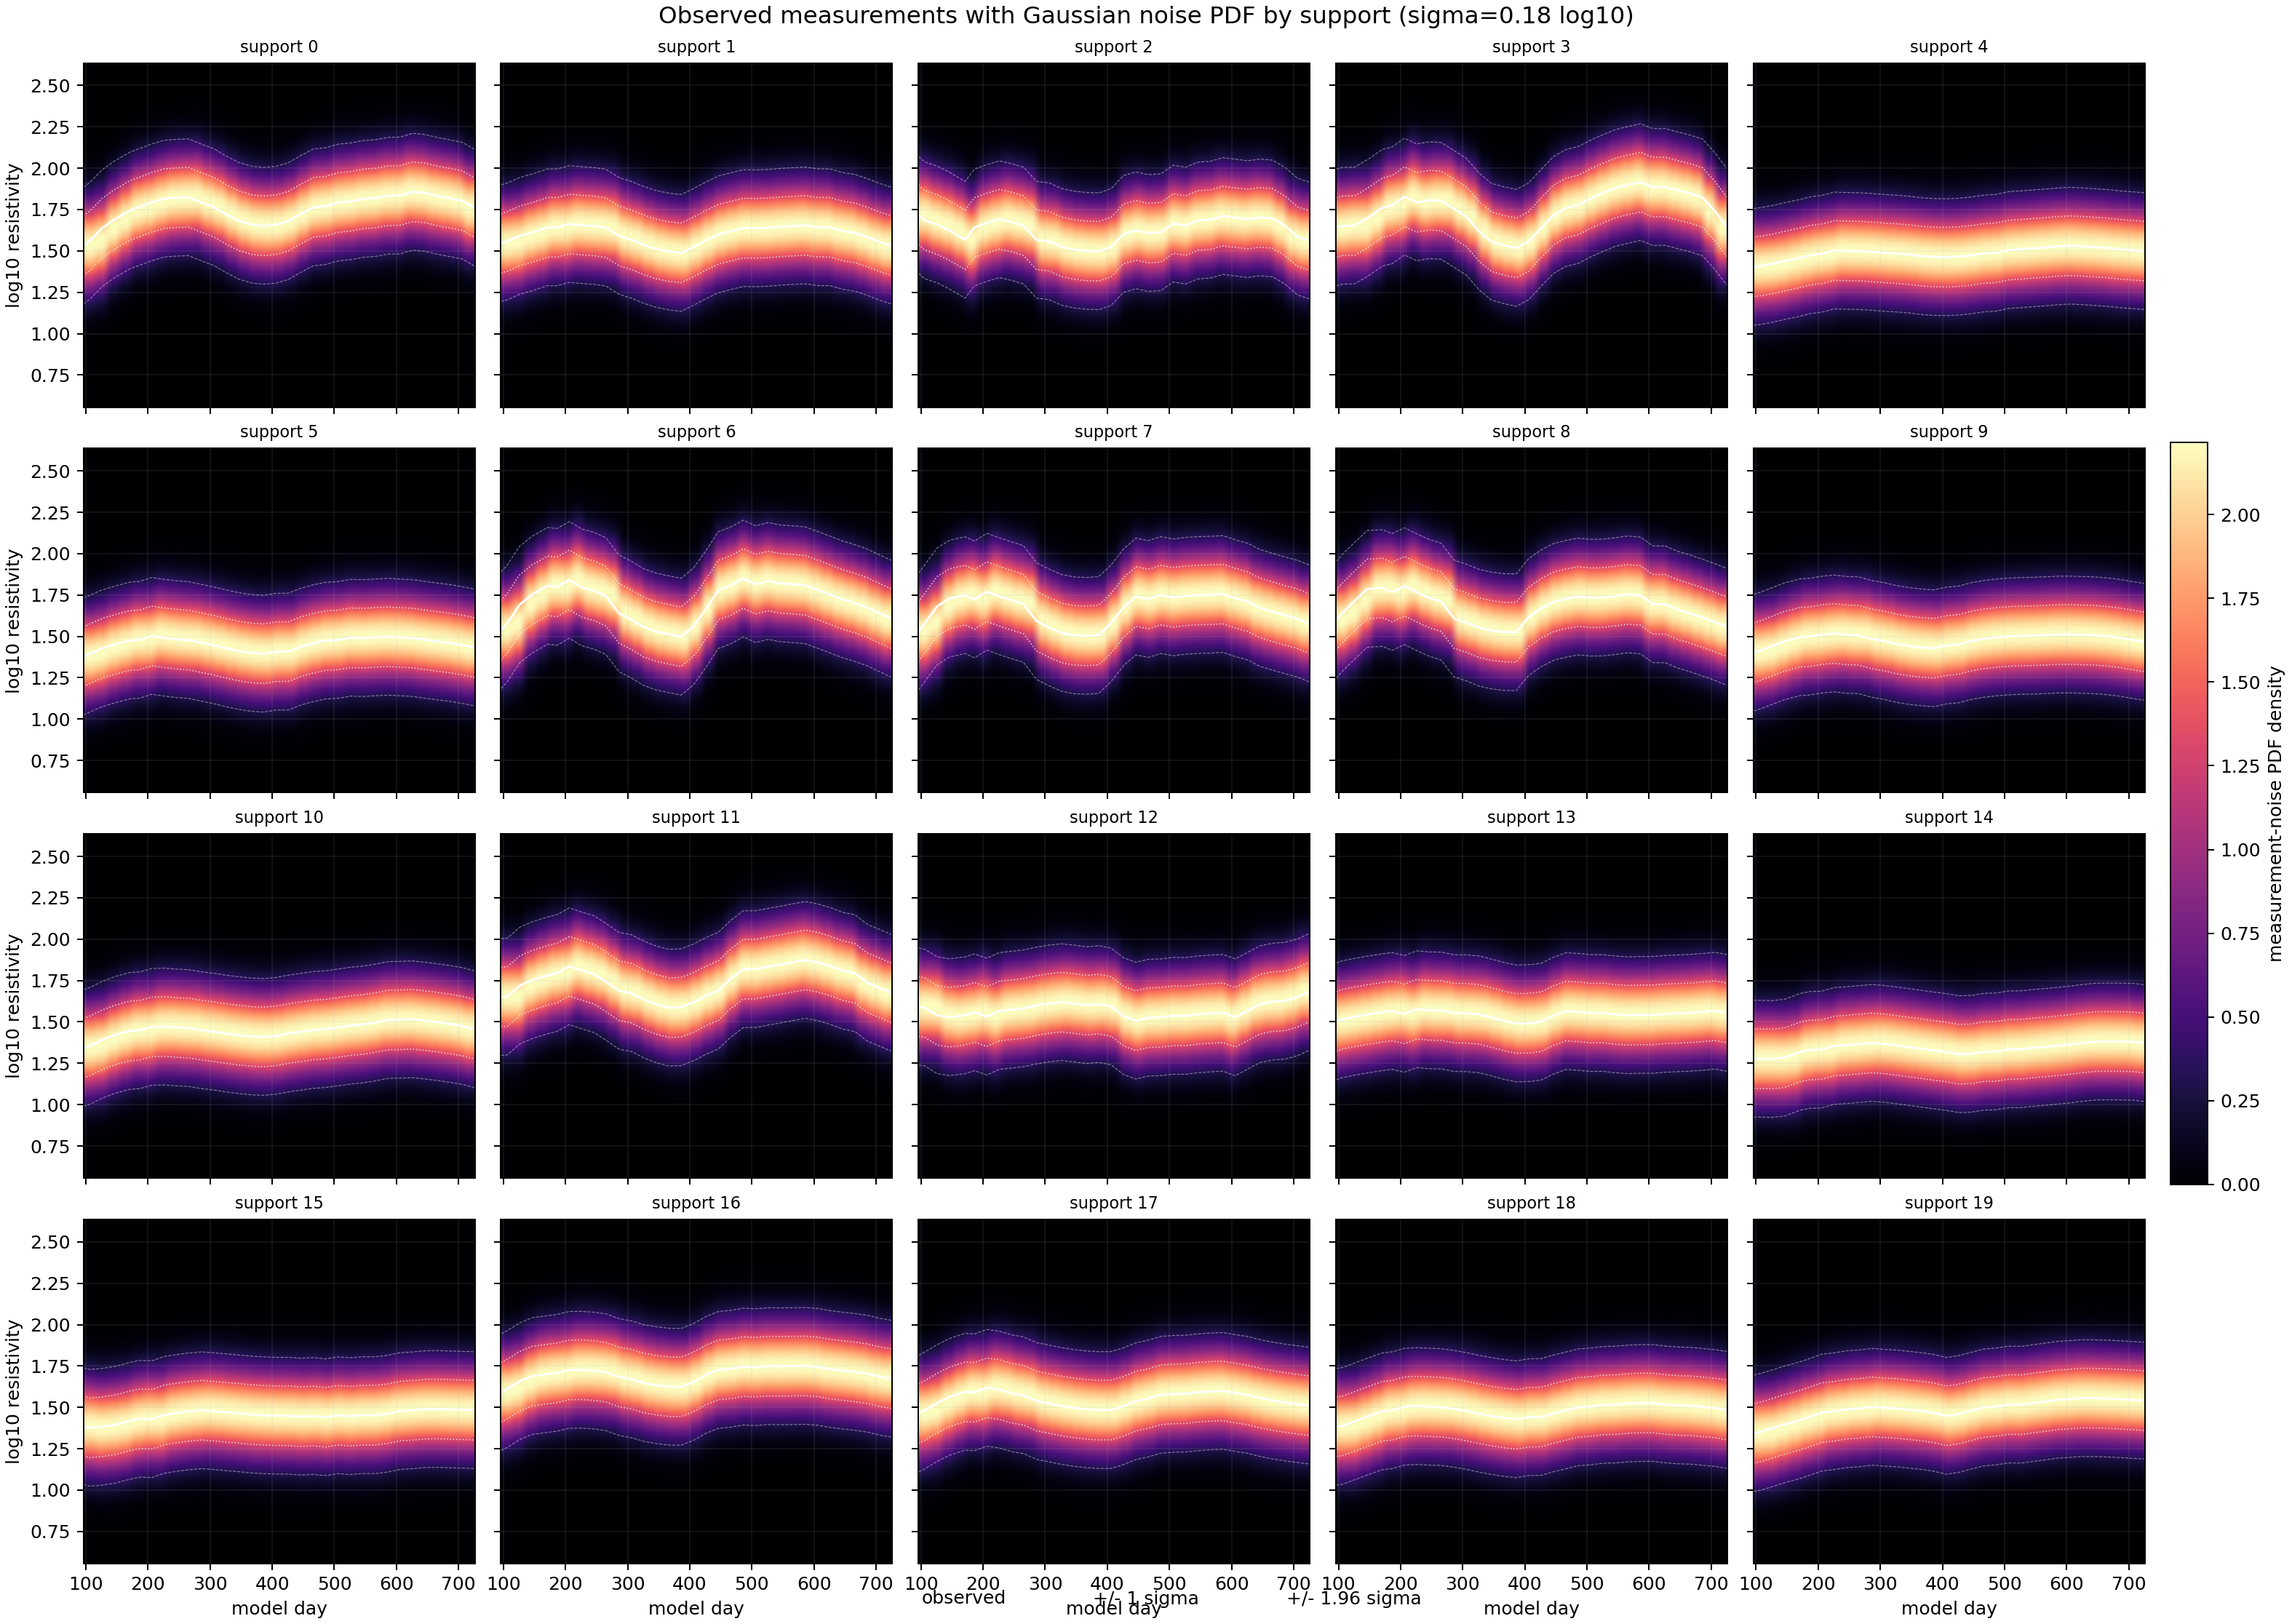
\includegraphics[width=\linewidth,height=0.70\textheight,keepaspectratio]{figures/posterior/measurement_noise_pdf_by_support_20plots.png}
\caption{Support-specific measurement-noise PDFs used for interpreting posterior predictive spread.}
\end{figure}


\clearpage
\section*{Field Posterior and Interpretation Limits}
The field posterior is a useful spatial summary of accepted exact candidates, but its interpretation is bounded by the data stream. Because this report assimilates only ERT over a limited window, the field statistics should be read as ERT-conditioned diagnostics under the chosen OGS model and local Archie transform, not as a fully validated hydro-mechanical material reconstruction.


\begin{table}[H]
\centering
\small
\begin{tabularx}{\linewidth}{>{\raggedright\arraybackslash}p{0.29\linewidth} X}
\toprule
\rowcolor{TableFill}\textbf{Item} & \textbf{Value}\\
\midrule
log10 permeability mean & min -24.89, median -16.29, max -6.539 \\
log10 permeability std & median 2.128 \\
porosity mean & min 0.0767, median 0.154, max 0.174 \\
porosity std & median 0.0105 \\
Field samples & 1,753 \\
\bottomrule
\end{tabularx}
\end{table}


\begin{figure}[H]
\centering
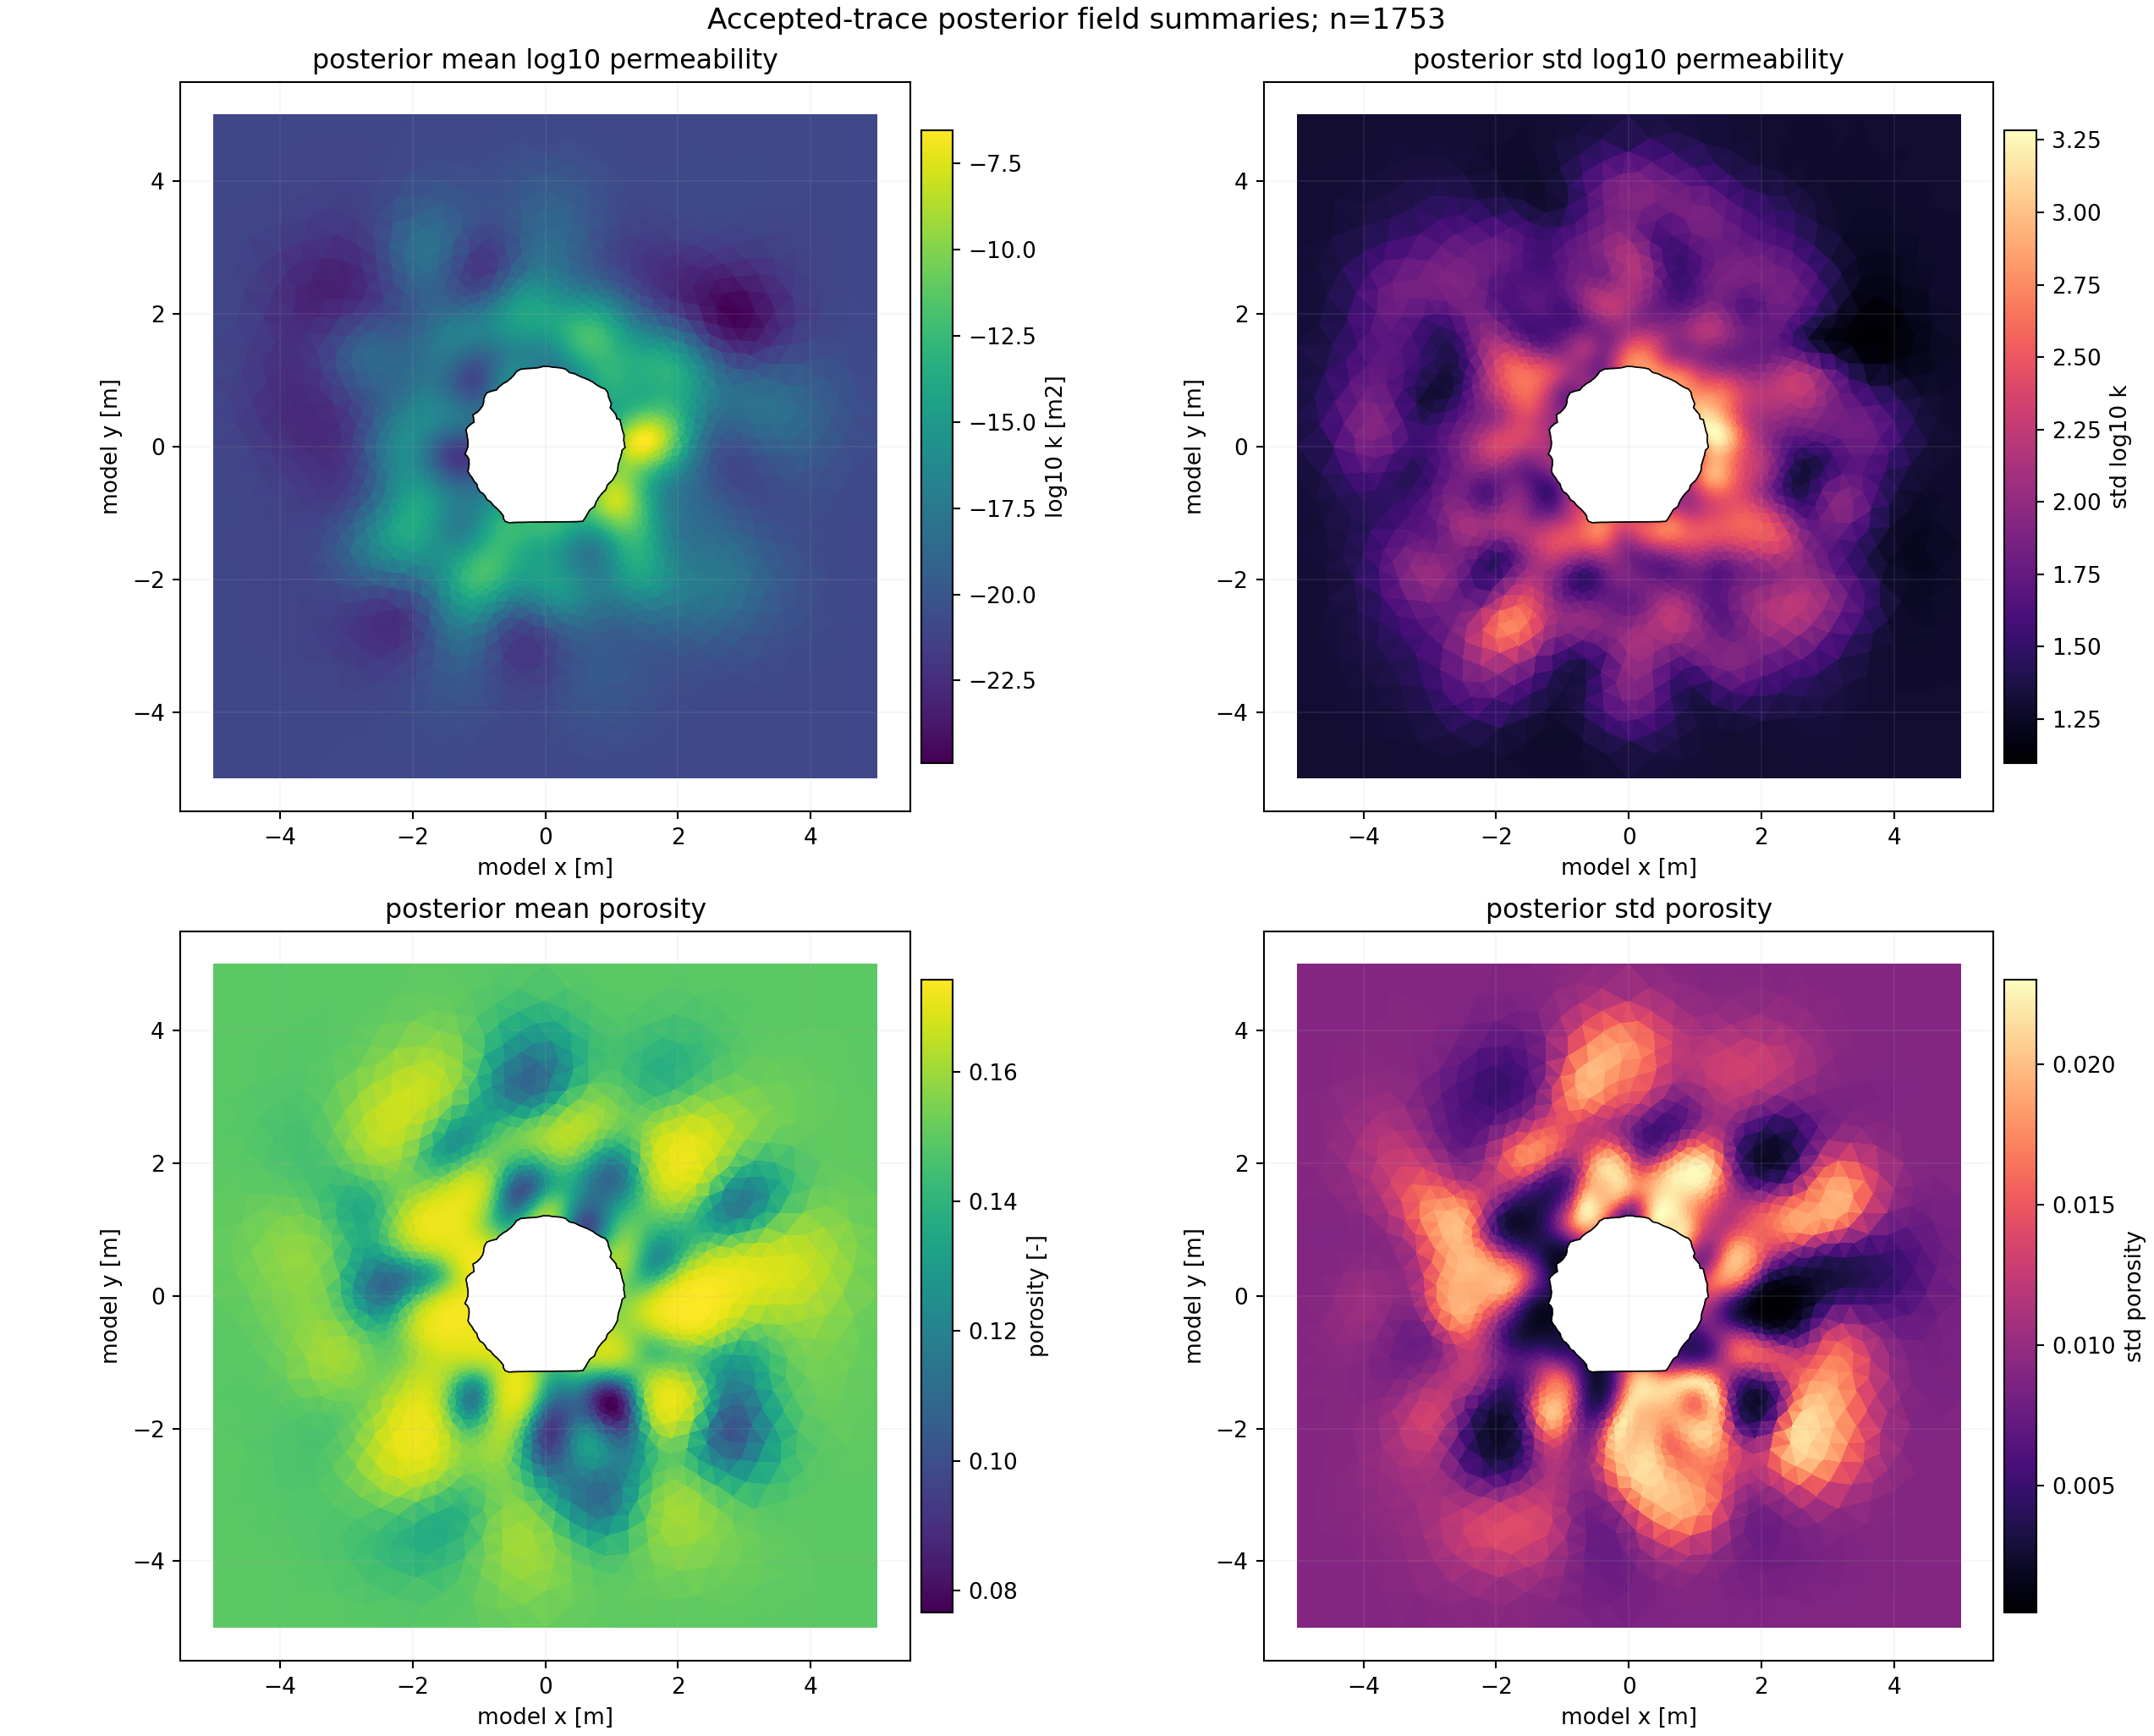
\includegraphics[width=\linewidth,height=0.68\textheight,keepaspectratio]{figures/posterior/posterior_field_mean_std.png}
\caption{Posterior field mean and standard deviation for permeability and porosity summaries.}
\end{figure}


\begin{figure}[H]
\centering
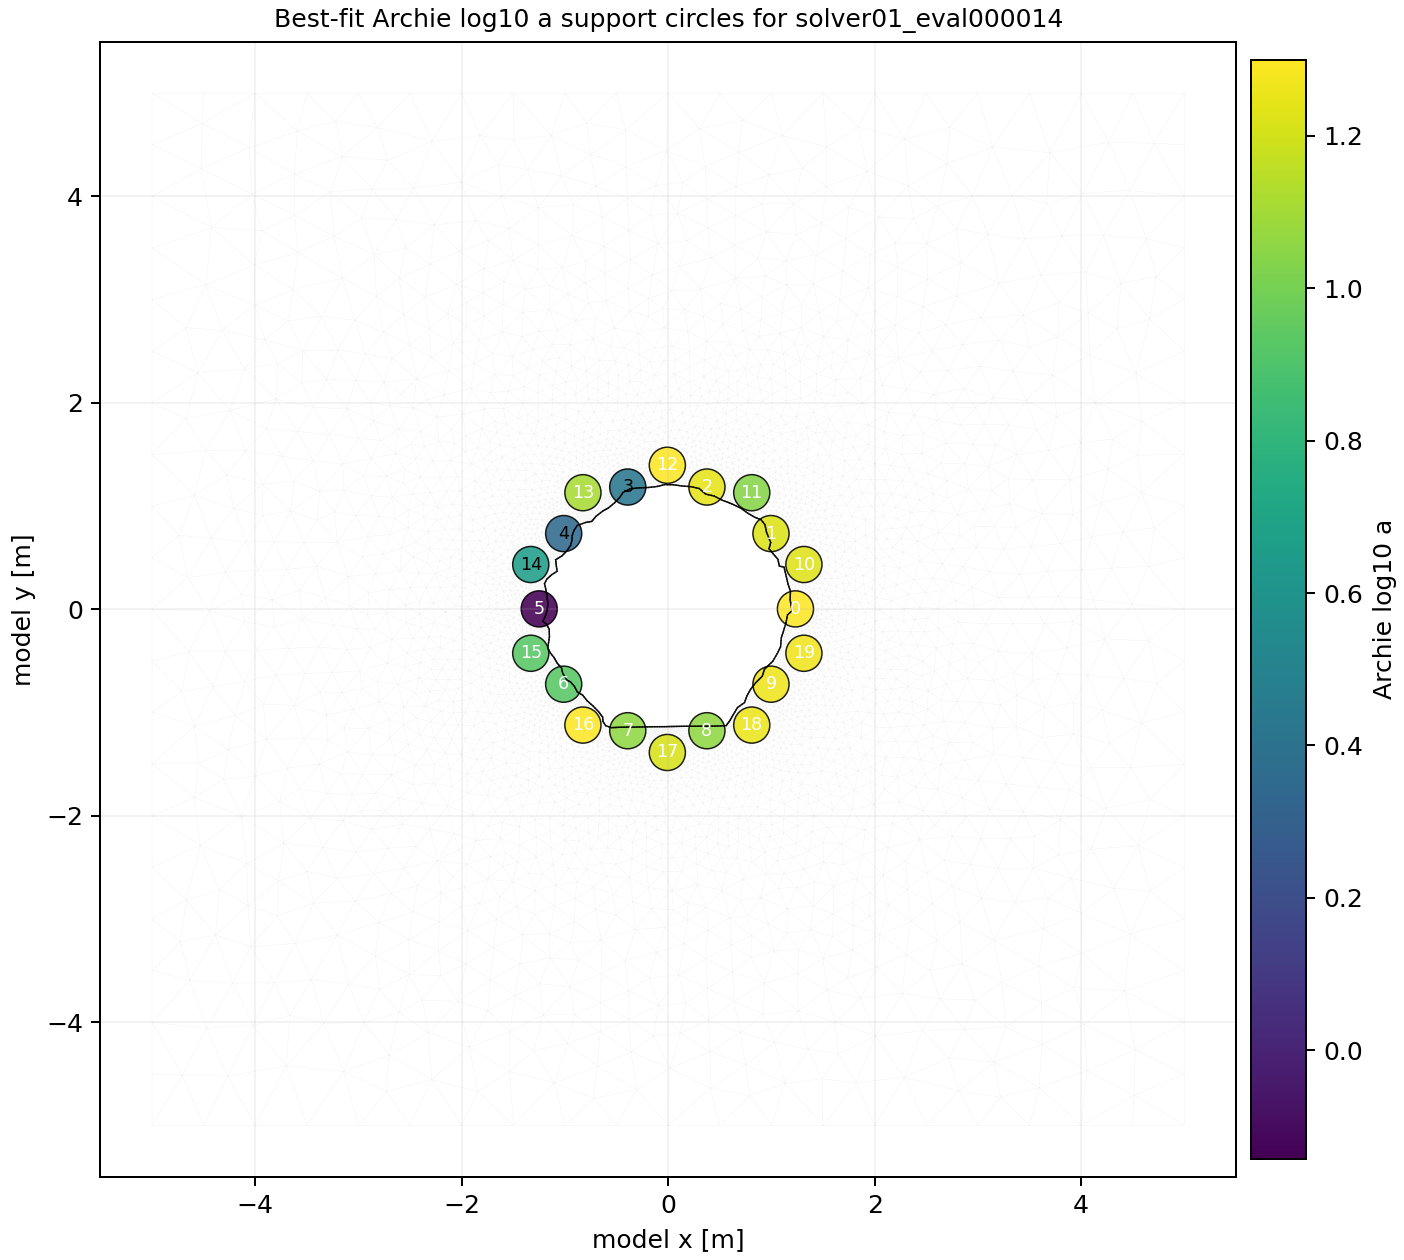
\includegraphics[width=\linewidth,height=0.66\textheight,keepaspectratio]{figures/posterior/posterior_best_fit_archie_log10_a_mesh_circles.png}
\caption{Spatial support layout colored by best-fit log10(a).}
\end{figure}


\begin{figure}[H]
\centering
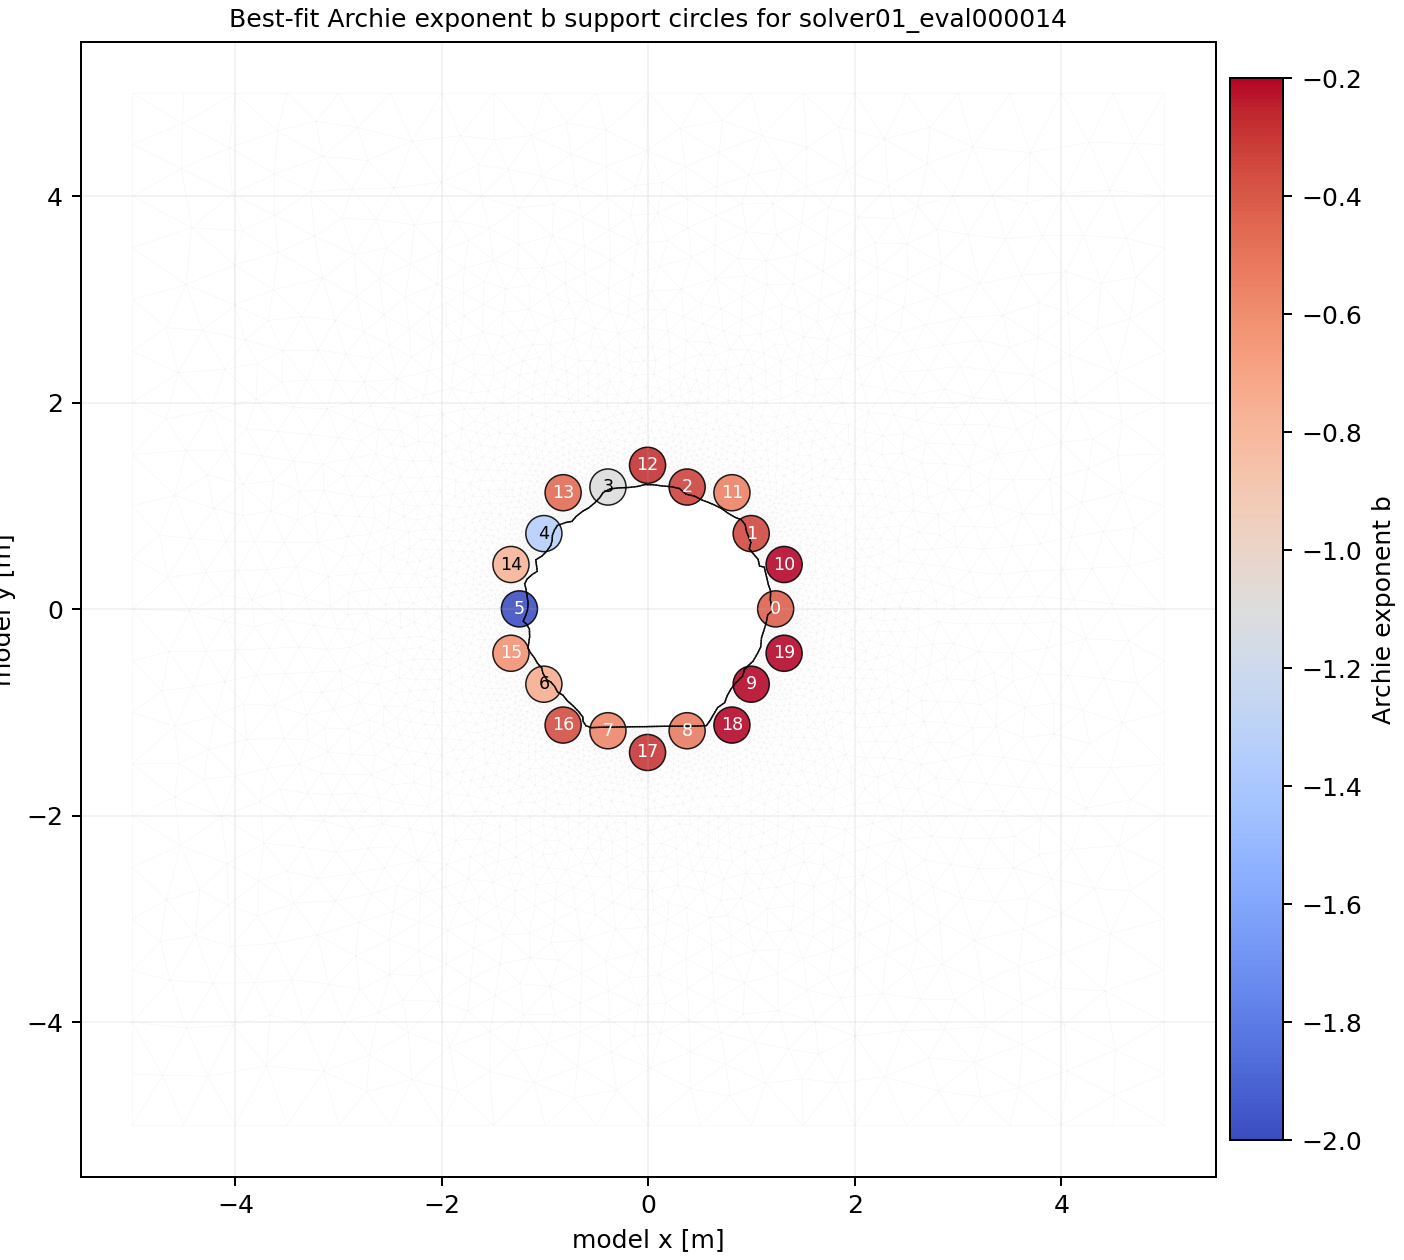
\includegraphics[width=\linewidth,height=0.66\textheight,keepaspectratio]{figures/posterior/posterior_best_fit_archie_exponent_b_mesh_circles.png}
\caption{Spatial support layout colored by best-fit Archie exponent b.}
\end{figure}


\clearpage
\section*{Reproducibility Notes}
The report is generated from saved run products rather than from sampler memory. The authoritative evidence is the manifest, candidate index, exact-training dataset manifest, residual diagnostics, posterior summaries, and figure directory under the run folder. This keeps the publication artifact compact while preserving traceability to the complete machine-readable record.


\begin{table}[H]
\centering
\small
\begin{tabularx}{\linewidth}{>{\raggedright\arraybackslash}p{0.29\linewidth} X}
\toprule
\rowcolor{TableFill}\textbf{Item} & \textbf{Value}\\
\midrule
Manifest & damh\_\allowbreak{}manifest.json \\
Candidate index & candidate\_\allowbreak{}index.csv and candidate\_\allowbreak{}index\_\allowbreak{}summary.json \\
Combined training dataset & combined\_\allowbreak{}training\_\allowbreak{}dataset\_\allowbreak{}manifest.json \\
Residual diagnostics & residual\_\allowbreak{}diagnostics\_\allowbreak{}summary.json and residual\_\allowbreak{}diagnostics\_\allowbreak{}by\_\allowbreak{}*.csv \\
Posterior summaries & DAMH\_\allowbreak{}ERT20\_\allowbreak{}POSTERIOR\_\allowbreak{}summary.json and DAMH\_\allowbreak{}ERT20\_\allowbreak{}POSTERIOR\_\allowbreak{}parameter\_\allowbreak{}summary.csv \\
Figures & report\_\allowbreak{}figures/ \\
Long-form image appendix & DAMH\_\allowbreak{}ERT20\_\allowbreak{}RESULTS\_\allowbreak{}REPORT\_\allowbreak{}FULL\_\allowbreak{}IMAGES.pdf \\
\bottomrule
\end{tabularx}
\end{table}


\vspace{0.3em}
\noindent\fcolorbox{BorderColor}{CautionFill}{%
\begin{minipage}{0.965\linewidth}
\small\textbf{Use boundary:} The current evidence does not assimilate RH/suction, NMR, direct pressure, deformation, or crack observations. Those streams can still be used for validation or future priors, but conclusions in this report should be read as ERT-conditioned over the reported time frame.
\end{minipage}}
\vspace{0.5em}


\end{document}
